% file thesis.tex
% Archivo thesis.tex
% Documento maestro que incluye todos los paquetes necesarios para el documento
% principal.

% Documento obtenido por un sinfin de iteraciones de administradores del LDC
% Estructura actual hecha por:
% Jairo Lopez <jairo@ldc.usb.ve>
% Actualizado ligeramente por:
% Alexander Tough 

\documentclass[oneside,12pt,letterpaper]{report}
\tolerance=1000  
\hbadness=10000  
\raggedbottom

% Paquetes para manejar graficos
\usepackage{epsf}
\usepackage[pdftex]{graphicx}
\usepackage{epstopdf}
\usepackage{epsfig}
% Simbolos matematicos
\usepackage{latexsym,amssymb}
% Paquetes para presentar una tesis decente.
\usepackage{setspace,cite} % Doble espacio para texto, espacio singular para
                           % los caption y pie de pagina

% Paquetes no utilizados para citas
%\usepackage{mcite} 
%\usepackage{draft} 

\usepackage{wrapfig}
\usepackage{alltt}

% Acentos 
\usepackage[spanish,activeacute]{babel}
\usepackage[spanish]{translator}
\usepackage[utf8]{inputenc}
\usepackage{color, xcolor, colortbl}
\usepackage{multirow}
\usepackage{subfig}
\usepackage[OT1]{fontenc}
\usepackage{tocbibind}
\usepackage{anysize}
\usepackage{listings}

% Para poder tener texto asiatico
%\usepackage{CJK}

% Opciones para los glosarios
\usepackage[style=altlist,toc,numberline,acronym]{glossaries}
\usepackage{url}
\usepackage{amsthm}
\usepackage{amsmath}
\usepackage{fancyhdr} % Necesario para los encabezados
\usepackage{fancyvrb}
\usepackage{makeidx} % En caso de necesitar indices.
\makeindex  % Necesitado para los indices

% Definiciones para definicions, teoremas y lemas
\theoremstyle{definition} \newtheorem{definicion}{Definici\'{o}n}
\theoremstyle{plain} \newtheorem{teorema}{Teorema}
\theoremstyle{plain} \newtheorem{lema}{Lema}

% Para la creacion de los pdfs
\usepackage{hyperref}

% Para resolver el lio del Unicode para la informacion de los PDFs
% En pdftitle coloca el nombre de su proyecto de grado/pasantia.
% En pdfauthor coloca su nombre.
\hypersetup{
    pdftitle = {Clustering de datos numericos por medio de algoritmos basados en poblacion e inteligencia colectiva},
    pdfauthor={Alexander De Sousa y Federico Ponte},
    colorlinks,
    citecolor=black,
    filecolor=black,
    linkcolor=black,
    urlcolor=black,
    backref,
    pdftex
}

\lstset{
   language=C,
   basicstyle=\footnotesize,
   keywordstyle=\textbf,
   showstringspaces=false,
   numbers=left,
   numberstyle=\footnotesize,
   mathescape=true,
   escapechar={\%},
   frame=bottomline,
   morekeywords={Mientras, Si, Sino, Para, Fin, FinSi, FinPara, FinMientras},
   commentstyle={\color{darkgrey}},
   literate={á}{{\'a}}1
            {é}{{\'e}}1
            {í}{{\'i}}1
            {ó}{{\'o}}1
            {ú}{{\'u}}1
            {ñ}{{\~n}}1
}

\usepackage{tikz}
\usetikzlibrary{positioning,shapes}
\usepackage{lmodern}
\usepackage{amsfonts}
\definecolor{darkgrey}{rgb}{0.4,0.4,0.4}
\usepackage{caption}
\DeclareCaptionFont{white}{\color{white}}
\DeclareCaptionFormat{listing}{\colorbox{gray}{\parbox{\textwidth}{#1#2#3}}}
\captionsetup[lstlisting]{format=listing,labelfont=white,textfont=white}



% Crea el glosario
\makeglossaries

% Incluye el glosario
\newacronym{as-h}{as-H}{proceso autosimilar con par\'{a}metro autosimilar $H$}

\newacronym{asie-h}{asie-H}{proceso autosimilar con par\'{a}metro autosimilar
$H$ e incrementos estacionarios}

\newacronym{aas-h}{aas-H}{proceso asint\'{o}ticamente autosimilar con
par\'{a}metro autosimilar $H$}


% Para crear la hoja escaneada de las firmas
\usepackage[absolute]{textpos}

% Pone los nombres y las opciones para mostrar los codigos fuentes
\lstset{language=C, breaklines=true, frame=single, showstringspaces=false,
        showtabs=false, numbers=left, keywordstyle=\color{black},
        basicstyle=\footnotesize, captionpos=b }
\renewcommand{\lstlistingname}{C\'{o}digo fuente}
\renewcommand{\lstlistlistingname}{\'{I}ndice de c\'{o}digos fuentes}

% Dimensiones de la pagina
\setlength{\headheight}{15pt}
\marginsize{3cm}{2cm}{2cm}{2cm}

% Se pueden omitir para que no compile ciertos capitulos.
\includeonly{header, intro, ssimilar, herramienta, resultados, conclusiones}

%%%%%%%%%%%%%%%%%%%%%%%%%%%%%%%%%%%%%%%%%%%%%%%%%%%%%%%%%%%%%%%%%%%%%%%%%%%
%%%%%%%%%%%%%%%%      end of preamble and start of document     %%%%%%%%%%%
%%%%%%%%%%%%%%%%%%%%%%%%%%%%%%%%%%%%%%%%%%%%%%%%%%%%%%%%%%%%%%%%%%%%%%%%%%%
\begin{document}

% Pagina de titulo
% Pagina de titulo
\begin{titlepage}
\begin{center}

% Upper part (aqui ya esta incluido el logo de la USB).

\includegraphics[scale=0.5,type=png,ext=.png,read=.png]{figures/cebolla} \\

% Encabezado
\textsc {\large UNIVERSIDAD SIM'ON BOL'IVAR} \\
\textsc{\bfseries DECANATO DE ESTUDIOS PROFESIONALES\\
COORDINACI'ON DE INGENIER'IA DE LA COMPUTACI'ON}

\bigskip
\bigskip
\bigskip
\bigskip
\bigskip
\bigskip
\bigskip
\bigskip
\bigskip

% Title/Titulo
% Aqui ponga el nombre de su proyecto de grado/pasantia larga
\textsc{\bfseries Clustering de datos numericos por medio de algoritmos basados en poblacion e inteligencia colectiva}

\bigskip
\bigskip
\bigskip
\bigskip
\bigskip

% Author and supervisor/Autor y tutor
\begin{minipage}{\textwidth}
\centering
Por: \\
Alexander De Sousa\\
Federico Ponte \\

\bigskip
\bigskip
\bigskip

Realizado con la asesor'ia de: \\
Emely Arra\'iz
\end{minipage}

\bigskip
\bigskip
\bigskip
\bigskip
\bigskip
\bigskip
\bigskip
\bigskip
\bigskip

% Bottom half
{PROYECTO DE GRADO \\ Presentado ante la Ilustre Universidad Sim'on Bol'ivar \\
como requisito parcial para optar al t'itulo de \\ Ingeniero en Computaci'on} \\

\bigskip
\bigskip
\vfill

% Date/Fecha 
{\large \bfseries Sartenejas, FECHA (MES de A\~NO)}

\end{center}
\end{titlepage}


% Pagina de acta final (vacio)
% Pagina del acta final
\begin{titlepage}
\begin{center}

% Upper part

\includegraphics[scale=0.5,type=png,ext=.png,read=.png]{figures/cebolla} \\

\textsc {\large UNIVERSIDAD SIM'ON BOL'IVAR} \\
\textsc{DECANATO DE ESTUDIOS PROFESIONALES\\
COORDINACI'ON DE INGENIER'IA DE LA COMPUTACI'ON}

\bigskip
\bigskip
\bigskip
\bigskip
\bigskip
\bigskip

% Title
\textsc{ACTA FINAL PROYECTO DE GRADO}

\bigskip
\bigskip

% Aqui coloca el nombre de su proyecto de grado/pasantia larga.
\textsc{\bfseries Clustering de datos numericos por medio de algoritmos basados en poblacion e inteligencia colectiva}

\bigskip
\bigskip
\bigskip
\bigskip

\begin{minipage}{\textwidth}
\centering
Presentado por: \\
% Aqui coloca su nombre.
\textsc{\bfseries Alexander De Sousa} \\
\textsc{\bfseries Federico Ponte} \\

\bigskip
\bigskip
\bigskip
\bigskip

Este Proyecto de Grado ha sido aprobado por el siguiente jurado examinador: \\

\bigskip
\bigskip

% Despues de cada line coloca el (los) nombre(s) de
% cada uno de los integrantes del jurado.
\line(1,0){200} \\
PROFESOR 1\\

\bigskip
\bigskip

\line(1,0){200} \\
PROFESOR 2 \\

\bigskip
\bigskip

\line(1,0){200} \\
PROFESOR 3 \\
\end{minipage}

\bigskip
\bigskip
\vfill

% Date/Fecha
{\large \bfseries Sartenejas, FECHA (dd/mm/aa)}

\end{center}
\end{titlepage}


\setcounter{secnumdepth}{3}
\setcounter{tocdepth}{4}

% Define encabezado numeros romanos y como se separan los captiulos y las
% secciones
\addtolength{\headheight}{3pt}
\pagenumbering{roman}
\pagestyle{fancyplain}

\renewcommand{\chaptermark}[1]{\markboth{\chaptername\ \thechapter:\,\ #1}{}}
\renewcommand{\sectionmark}[1]{\markright{\thesection\,\ #1}}

\onehalfspacing

\lhead{}
\chead{}
\rhead{}
\renewcommand{\headrulewidth}{0.0pt}
\lfoot{}
\cfoot{\fancyplain{}{\thepage}}
\rfoot{}


% Pagina de resumen
\vspace{5 mm}

\setcounter{page}{4}
\begin{center}
	{\bf Resumen}
\end{center}

\vspace{5 mm}

La agrupación de datos (\emph{data clustering}) es el proceso de particionar una
colección de datos en conjuntos de clases significativas, llamadas \emph{clusters},
donde los objetos de una clase comparten ca\-rac\-te\-rís\-ti\-cas comunes. En este trabajo,
se presenta un estudio comparativo de cinco metaheurísticas basadas en población
e inteligencia colectiva (\emph{algoritmo genético}, \emph{optimizador de enjambre
de partículas}, \emph{evolución diferencial}, \emph{algoritmo de abeja} y
\emph{algoritmo de clustering de hormigas}) para resolver el problema de \emph{data
clustering} en calidad de soluciones finales. Los datos usados para el estudio son
de tipo numérico, comúnmente utilizados en la literatura afín. Del estudio se
llega a la conclusión que para resolver el problema de \emph{clustering} de datos
numéricos se deben utilizar el \emph{algoritmo genético} o el \emph{algoritmo de
abeja}, ambos hibridados con la heurística \emph{K-means} como método de mejoramiento
de las soluciones finales.

\newpage



% Pagina de dedicatoria (opcional)
\setcounter{page}{5}

\vspace*{8cm} 
\pdfbookmark[0]{Dedication}{dedication} % Sets a PDF bookmark for the dedication
\begin{center} 
\large DEDICATORIA
\end{center}
\newpage


% Pagina de agradecimientos (opcional)
\setcounter{page}{6}

\chapter*{Agradecimientos
\markboth{Agradecimientos}{Agradecimientos}}
A todas las personas que aportaron su granito de arena en la realización de este
proyecto de grado, en especial, nuestra tutora.


% Crea la tabla de contenidos
\tableofcontents

% Crea la lista de cuadros
\listoftables

% Crea la lista de figuras
\listoffigures

% Crea la lista de codigos fuentes
%\lstlistoflistings

\clearpage

% Define encabezado en numeros arabicos  
\pagenumbering{arabic}

\fancyhf{} % Redefine el encabezado 
\lhead{}
\chead{}
\rhead{\fancyplain{}{\thepage}}
\renewcommand{\headrulewidth}{0.0pt}
\lfoot{}
\cfoot{}
\rfoot{}

\doublespacing


% Incluye los archivos deseados - El contenido de
% su proyecto de grado/pasantia larga.
 \addcontentsline{toc}{chapter}{Introducci\'on}

% Titulo de la introduccion.
\begin{center}
	{\bf Introducci\'on} \label{chap:intro}
\end{center}

% Contenido de la introduccion.

\label{sect:motivacion}
%Puedes quitar esto(es opcional)
\vspace{5 mm}

En la Universidad Sim\'on Bol\'ivar es dictada la materia electiva
Dise\~no de Algoritmos II, en la cual se enseñan diversas metaheur\'isticas.
El curso es dividido en grupos (normalmente en parejas) y a cada uno se le asigna un problema 
de optimizaci\'on NP-hard para resolver mediante estos m\'etodos. Uno de \'estos es Data Clustering.
Consiste m\'etodo de crear grupos de objetos,
de tal manera que los objetos dentro de un cluster sean similares y 
en clusters distintos sean diferentes. \cite{GaChJi2007}

%Puedes quitar esto(es opcional)
\vspace{5 mm}

\label{sect:justificacion}
%Puedes quitar esto(es opcional)
\vspace{5 mm}

Se sabe que hoy en d\'ia hay muchos avances y usos del reconocimiento de im\'agenes.
Ejemplos son Google Goggles, diversos m\'odulos de JDownloader con el objetivo de reconocer
captchas, reconocimiento de caras por parte de las c\'amaras, etc. Un algoritmo de
Data Clustering sirve como entrada para un modelo basado en sistemas de
reconocimiento de objetos. Tambi\'en el poder encontrar patrones escondido en
conjuntos de datos es muy \'util: una empresa podr\'ia mejorar su ventas.

%Puedes quitar esto(es opcional)
\vspace{5 mm}

\label{sect:planteamiento}
%Puedes quitar esto(es opcional)
\vspace{5 mm}

Actualmente existe una ardua investigaci\'on en diversas metaheur\'isticas para
resolver diversos problemas optimizaci\'on. La idea es obtener en un tiempo
considerable una respuesta \'optima o lo m\'as cercano posible a \'esta. Por
ello muchos cient\'ificos han empezado a inspirarse en la naturaleza.
Una profunda obsevaci\'on en la relaci\'on subyacente 
entre \'esta y optimizaci\'on ha llevado al desarrollo de nuevos paradigmas
para lograr este objetivo\cite{SwAjAm2009}. De ac\'a surgen las basadas en poblaci\'on e inteligencia
colectiva.

Los m\'as prominentes y prometedores son el algoritmo g\'enetico, abeja, DE, hormiga
y PSO. Todos constan de un grupo de individuos que van a ir modificandose a trav\'es
del tiempo. La forma en que se den estos cambios depende de cada algoritmo.

%Puedes quitar esto(es opcional)
\vspace{5 mm}

\label{sect:objetivo_general}
%Puedes quitar esto(es opcional)
\vspace{5 mm}

El objetivo principal es la implementaci\'on de \'estas cinco metaheur\'isticas
y el K-means, el algoritmo m\'as famoso para data clustering, para ver la calidad
de cada uno y compararlos entre si. \'Esta debe ser eficiente, rapida y flexible
con el objetivo de que pueda ser usada a futuro por otras personas y lograr
comprar los algoritmos de la forma m\'as efectiva.


%Puedes quitar esto(es opcional)
\vspace{5 mm}

\label{sect:objetivos_especificos}
%Puedes quitar esto(es opcional)
\vspace{5 mm}

El programa debe tener la capcidad de leer archivos en formato CSV e im\'agenes
en formato PNG y TIFF (las im\'agenes son datos n\'umericos). La salida tiene que ser
concorde al tipo de cada archivo, para un csv un archivo de texto y
en el otro caso una imagen con un color para cada grupo creado. Es necesario que
el lenguaje que se use tenga la capcidad de compilar a c\'odigo de m\'aquina
en vista que se busca eficiencia en tiempo.

Para comparar las diversas metaheur\'sticas es esencial tener una m\'etrica com\'un
con ese fin. Adem\'as se debe colocar un limite de tiempo en las corridas para 
obtener una buena soluci\'on en un tiempo considerable.



\chapter{Métodos de Optimización} \label{chap:mopt}

El objetivo de la optimización es buscar valores para un conjunto de
parámetros que maximicen o minimicen la función objetivo del problema de modo
que se satisfagan las restricciones del mismo. Una solución factible es una
elección de valores para el conjunto de parámetros que satisfacen todas las
las restricciones del problema. Las soluciones factibles con mejores valores de
función objetivo son llamadas soluciones óptimas.

    Las técnicas de optimización son usadas diariamente para planificación
industrial, administración de recursos, programación de horarios, toma de
decisiones, agrupación no supervisada de datos, etc. Por lo tanto, las técnicas de
optimización son ampliamente usadas en muchos campos como ingeniería, industria,
medicina y negocios. La investigación en el campo de la optimización es bastante
activa y nuevos métodos de optimización son desarrollados regularmente \cite{GO_1}.

    La optimización abarca tanto problemas de maximización como de minimización.
Cualquier problema de maximización puede ser convertido en un problema de
minimización al tomar la inversa de la función objetivo del mismo y
viceversa. En general, un problema de optimización puede ser definido como:

    Sea $S$ el espacio de soluciones y $d$ la dimensión del mismo donde:
\begin{itemize}
    \item $f: S \rightarrow \mathbb{R}$ es la función objetivo de maximización
del problema.
    \item $S \subseteq \mathbb{R}^d$
\end{itemize}
    entonces se debe encontrar $x^* \in S$ tal que:
\begin{itemize}
    \item $f(x^*) \geq f(x), \forall x \in S$ si se desea una función maximizadora.
    \item $f(x^*)^{-1} \leq f(x)^{-1}, \forall x \in S$, si se desea una función
minimizadora.
\end{itemize}

    El valor de $f(x^*)$ (ó $f(x^*)^{-1}$) es llamado óptimo global. La
optimización global es la tarea de encontrar la solución global óptima. En
general, existen soluciones que son localmente óptimas pero no globalmente
óptimas. Por lo tanto los problemas de optimización global son difíciles de
resolver de manera exacta. En el contexto de problemas combinatorios, estos
problemas son frecuentemente NP-hard \cite{GO_2}. Un buen algoritmo de
optimización global encontrará $x^*$ sin importar el punto inicial $x_0 \in S$.

    Algunos ejemplos de problemas de optimización global son \cite{GO_2}:
\begin{itemize}
    \item Problemas combinatorios: donde la función lineal o no-lineal es definida
sobre un conjunto finito, pero bastante grande de soluciones, Por ejemplo,
agrupación no supervisada de datos, programación de horarios, entre otros.
    \item Problemas generales sin restricciones: donde se define una función
no-lineal sobre un conjunto de valores reales sin restricciones.
    \item Problemas generales con restricciones: donde se define una función
no-lineal sobre un conjunto de valores reales con restricciones.
\end{itemize}

\subsection{Algoritmos Tradicionales de Optimización}

    Los algoritmos de optimización tradicionales usan métodos exactos para
encontrar la mejor solución. Si el problema tiene solución, entonces estos algoritmos
son capaces de encontrar la solución óptima global.

    Algunos de estos algoritmos son \cite{TA_1}:
\begin{itemize}
    \item \emph{Fuerza bruta}: comparan todas las soluciones del espacio de
soluciones de modo que encontrar la solución global óptima esté garantizada. Sin
embargo, a medida que crece el espacio de soluciones el costo de los algoritmos
de fuerza bruta incrementa. Por lo tanto no son apropiados para la clase de
problemas pertenecientes al grupo NP-hard.
    \item Programación lineal: sirven para problemas donde una variable depende
de una o más variables de manera lineal:
\begin{center}
    $f(X_1, X_2, \cdots, X_n) = a_1 \cdot X_1 + a_2 \cdot X_2 + \cdots + a_n \cdot X_n$
\end{center}

    En otras palabres, $f(X_1, X_2, \cdots, X_n)$ (función objetivo del algoritmo)
puede ser expresada como una combinación lineal de las variables
$X_1, X_2, \cdots, X_n$. 
    \item Programación dinámica: funciona bajo el principio de encontrar una
solución total, operando en un punto intermedio que está entre la ubicación actual
y la ubicación final. El procedimiento es recursivo y cada punto intermedio es una
función de los puntos ya visitados. Una vez alcanzada la meta, se puede reconstruir
de manera inversa el camino óptimo generado por el algoritmo.
\end{itemize}

\subsection{Algoritmos Estocásticos}

    Los algoritmos estocásticos son usados para hallar soluciones
cercanas al óptimo global para problemas NP-hard en tiempo polinomial. Estos
algoritmos logran su objetivo al asumir que las soluciones buenas están
cercanas unas de otras en el espacio de búsqueda. Sin embargo, a diferencia de
los algoritmos tradicionales, estos podrían no encontrar la solución óptima
global \cite{PSO_0}.

    Las ventajas de los algoritmos estocásticos tienen varias
ventajas comparados con otros algoritmos \cite{SA_1}:
\begin{itemize}
    \item Son generalmente fáciles de implementar.
    \item Pueden ser usados eficientemente en paralelo.
    \item No requieren de la función de definición del problema para ser
continuos.
    \item Generalmente pueden encontrar la solución óptima o cercana a la
óptima.
    \item Sirven para problemas discretos y combinatorios.
\end{itemize}

    Algunos algoritmos estocásticos son \cite{PSO_0}:
\begin{itemize}
    \item Hill-Climbing: consiste en tomar una solución potencial aleatoria del
problema $x_0$ y buscar en la vecindad $N_0$ de $x_0$ una nueva mejor solución
al problema. Si se encentra un $x_1 \in N_0$ tal que $x_1$ es mejor que $x_0$,
entonces $x_1$ es la nueva solución potencial y se repite el procedimiento que
se hizo con $x_0$. Si no se encuentra una solución $x_1 \in N_0$ tal que
$x_1$ es mejor que $x_0$, entonces $x_0$ es la mejor solución encontrada por el
algoritmo \cite{TA_1}.
    \item Simulated Annealing: consiste en tomar una solución aleatoria del
problema $x_0$ y un valor pequeño $\epsilon$ para perturbar las soluciones.
Si $x_0 + \epsilon$ es mejor que $x_0$, entonces la nueva mejor solución es 
$x_0 + \epsilon$ y se repite el procedimiento. Sino, la solución $x_0$ será
perturbada con una probabilidad que se va decrementando a medida que avanza la
ejecución del algoritmo para seguir buscando \cite{SA_2}.
    \item Búsqueda Tabú: consiste en una búsqueda heurística que mantiene una
lista de memoria tabú de las soluciones previamente visitadas, de modo que se
mejore el proceso de búsqueda. La lista tabú es usada como una guía de
movimiento de una solución a la siguiente para evitar ciclos \cite{SA_5} y que 
se quede atrapado en un óptimo local. Inicialmente, Tabú comienza su búsqueda
con una solución elegida aleatoriamente. A partir de la solución actual se
generan un conjunto de soluciones de prueba. La mejor solución de prueba se
coloca como solución actual si no está en la lista tabú o, si está en la lista
tabú, pero satisface el criterio de aspiración. Una solución satisface un
criterio de aspiración si está en la lista tabú y es la mejor solución
encontrada hasta el momento. Este proceso se repite hasta que el criterio de
parada se satisfaga \cite{SA_3}\cite{SA_4}.
\end{itemize}
    
\subsection{Algoritmos Evolutivos (EA)}
    Los algoritmos evolutivos (\emph{EAs}) son métodos de búsqueda estocásticos de
propósito general que simulan la selección natural y la evolución de los
organismos biológicos. Los \emph{EAs} difieren de otros métodos de optimización,
como Hill-Climbing y Simulated Annealing, en que los \emph{EAs} mantienen una
población de soluciones potenciales a un problema y no sólo una solución.

    En general, todos los EAs funcionan de la siguiente manera:
\begin{itemize}
    \item Se inicializa una población de individuos (soluciones potenciales al
problema).
    \item La calidad de cada solución está dada por la función de
\emph{fitness}, que no es más que la función objetivo del algoritmo.
    \item En cada iteración, se aplica un proceso de selección para formar a la
población de la siguiente iteración. Este proceso está orientado a elegir
individuos que tengan una buen valor de \emph{fitness}.
    \item Los individuos son alterados a través de dos procesos: una
transformación unaria (mutación) y una transformación de orden superior (cruce o
crossover) \cite{PSO_0}.
    \item Se espera que la mejor solución encontrada esté cerca del óptimo.
\end{itemize}

    Se llaman operadores evolutivos a las transformaciones unaria y de orden
superior. Los operadores evolutivos más comunes son \cite{PSO_0}:
\begin{itemize}
    \item \textbf{Selección}: es un operador que elige a uno o más individuos para
aplicarles los otros operadores evolutivos. Las estrategías varían desde elegir
a los mejores individuos de la población hasta elegir a los mejores individuos
de un conjunto elegido aleatoriamente.
    \item \textbf{Mutación}: es un operador que modifica a un individuo a través
de un pequeño cambio para generar un nuevo individuo. El objetivo principal de
la mutación es introducir diversidad ``genética'' para evitar quedar atascado en
un óptimo local.
    \item \textbf{Recombinación o Cruce}: es un operador que combina a dos o más
individuos para generar nuevos individuos. El principal objetivo del cruce es
explorar nuevas áreas en el espacio de búsqueda.
    
\end{itemize}

\begin{lstlisting}[float=h, caption=Algoritmo Evolutivo General]
- Inicializar a cada individuo de la población.

- Evaluar el %\emph{fitness}% de cada individuo de la población.

- Mientras no se satisfaga el criterio de parada:

    - Aplicar el proceso de %\textbf{selección}%.

    - Alterar los individuos usando los operadores de %\textbf{cruce}% y
    %\textbf{mutación}%.

    - Evaluar el %\emph{fitness}% de cada individuo de la población.

- FinMientras.

\end{lstlisting}

    Las cuatro técnicas evolutivas más relevantes son \cite{PSO_0}:
\begin{itemize}
    \item La \textbf{programación genética} que es usada para buscar el
programa más eficiente para resolver un problema específico.
    \item La \textbf{programación evolutiva} que es usada generalmente para
optimizar funciones reales continuas. No utilizan el operador de recombinación.
    \item Las \textbf{estrategias evolutivas} que son usadas para optimizar
funciones reales continuas. Usa los operadores de selección, cruce y mutación.
No solo optimiza a la población, sino también al proceso de optimización al
evolucionar los parámetros de estrategia.
    \item Los \textbf{algoritmos genéticos} que son generalmente usados para
optimizar problemas combinatorios.
\end{itemize}

    Los algoritmos evolutivos pueden evitar quedar atrapados en un óptimo local
al tener varias soluciones potenciales al mismo tiempo y pueden encontrar
frecuentemente las soluciones óptimas globales. Sin embargo, existe cierto
riesgo de que no converjan a la solución global óptima \cite{SA_4}.

\subsection{Algoritmo Genético (GA)}

Imita la evoluci\'on gen\'etica de las especias. Un aspecto importante es que
explora varias soluciones a la vez, y no se enfoca en s\'olo una. A medida que
se ejecuta, las soluciones, tambi\'en llamadas individuos o cromosomas, 
toman parte en un proceso reporoductivo, donde interactuan, mezclan y producen
hijos que retiene algunas caracter\'isticas de sus padres. \'Este proceso
que conlleva a la creaci\'on de nuevas soluciones (hijos) esta basada en
la selecci\'on, cruce y mutaci\'on\cite{DoGeGr2007}.

Los cromosomas se pueden codificarse de bastantes modos, donde el m\'as 
com\'un es mediante strings de n\'umeros binarios (100101110101). El modo en
que se codifiquen tamb\'en depende del problela.


El pseudoc\'odigo es de la siguiente manera (hay m\'as interpretaciones posibles):

\begin{lstlisting}[float=h, caption=Algoritmo General Genetico]
    - Inicialización.
    Mientras no se cumpla el criterio de parada.
        Si rand(0,1) <= pc
            - Selección.
            - Cruce.
            Si rand(0,1) <= pm
                - Mutación.
            FinSi
            Si los hijos tiene mejor función objetico que los papas.
                - Colocarlos en la población y eliminar a los padres.
            FinSi
        FinSi
    FinMientras
\end{lstlisting}

Donde pc es la probabilidad de cruce, pm la de mutaci\'on y rand(0,1)
es una funci\'on que devuelve un n\'umero aleatorio entre 0 y 1. Y el resto
se define como :

\begin{itemize}

\item {\bf Inicializaci\'on:} Los par\'ametros son fijados y se
crean los cromosomas de la poblaci\'on.

\item {\bf Selecci\'on:} Consiste en elegir los padres. 

En \cite{GePo2010} comentan sus formas de implementar m\'as comunes:

\begin{itemize}

\item Tomar m\'as cuenta los individuos
con mejor funci\'on objetvo. Para ello se puede usar el m\'etodo bastante conocido
llamado roulette-wheel. 

\item Selecci\'on por torneo, en
donde un conjunto de cromosomas $\tau$ son elegidos y comparados, los mejores
son elegidos para ser padres. 

\end{itemize}

\item {\bf Cruce:}

Consiste en replazar los genes de uno de los padres por los del otro. Se puede hacer
de la siguiente manera continuando \cite{GePo2010}:

\begin{itemize}

\item {\bf De un punto:} Si se tienen dos padres de longitud $X$, se va a tomar
un punto entre $[1,X-1]$ y se generan dos hijos de la siguiente manera: el primero,
de 0 al punto con los genes del primer padre y del punto a $X$, y el segundo es 
lo contrario.

Si se tienen los padres [1 3 2 4 6]  y [5 1 3 6 2] y el punto 
de crude es el 2, entonces se generan los siguientes hijos:

[1 3 3 6 2] y [5 1 2 4 6]

\item {\bf De dos punto:} Ac\'a se eligen dos puntos distintos que cumplan con la 
misma condici\'on como en el de un punto. Para explicar es mucho mas sencillo
mediante un ejemplo:

Si se tienen los padres [1 3 2 4 6]  y [5 1 3 6 2] y los puntos 
de crude son el 2 y 4, entonces se generan los siguientes hijos:

[1 3 3 6 6] y [5 1 2 6 2]

De esta misma forma se puede extender para m\'as puntos.

\end{itemize}

\item {\bf Mutaci\'on:}

Consiste en modificar uno de los cromosomas bien sea de la poblaci\'on
o uno de los hijos generados. Un caso bastante com\'un es el de usar una m\'ascara
cuando los cromosomas son binarios\cite{GePo2010}.

Por su lado en esa misma referencia se comenta que para clustering se pueden usar los siguientes:

\begin{itemize}

\item En el caso que se use la representaci\'on binaria, alternar los bits es un
buen operador.

\item Cuando la representaci\'on es de enteros de etiquedas, se puede cambiar
el cluster al cual pertenece uno de los objetos.

\item Remplazar uno de los centroides por uno de los objetos pertenecientes a ese
cluster.

\end{itemize}

\end{itemize}

\subsection{Optimizador de Enjambre de partículas (PSO)}

    Un optimizador de enjambre de partículas (\emph{PSO}: Particle Swarm Optimizer)
es un algoritmo poblacional de optimización estocástico modelado a partir de la
simulación del comportamiento social de las bandadas de aves \cite{PSO_1}
\cite{PSO_2}.

    En un sistema PSO, un enjambre (swarm) de individuos, llamados partículas, se
mueven a través de un espacio de búsqueda. Cada partícula representa una
solución candidata al problema de optimización. La posición de  cada partícula
es influenciada por la mejor posición visitada por ella (su propia experiencia)
y la posición de la mejor partícula en su vecindad (la experiencia conjunta de
todas las partículas de su vecindad). Cuando la vecindad de una partícula es
el enjambre completo, la mejor posición en su vecindad se refiere a la mejor
partícula global y el algoritmo resultante es el \emph{gbest PSO} (Global Best
PSO). Por otra parte, cuando se utilizan vecindades más pequeñas, el algoritmo
generalmente se refiere al \emph{lbest PSO} (Local Best PSO) \cite{PSO_0}.

    Las principales diferencias entre el \emph{PSO} y los \emph{EAs} son
\cite{PSO_0}:
\begin{itemize}
    \item El \emph{PSO} se ve influenciado más en la experiencia social que la
supervivencia del más apto, como ocurren el los \emph{EAs}.
    \item En el \emph{PSO}, cada individuo se ve beneficiado de su historia. Esto
no ocurre en los \emph{EAs}.
\end{itemize}

\subsubsection{Características de las partículas}

    En el \emph{PSO}, cada partícula tiene una serie de características
\cite{PSO_0}:
\begin{itemize}
    \item $x_i$: La posición actual de la partícula $i$. Dependiendo del
problema, la posición de cada partícula tendrá una o más dimensiones.
    \item $v_i$: La velocidad actual de la partícula $i$. La dimensión de la
velocidad dependerá de la dimensión de la posición de la partícula.
    \item $y_i$: La mejor posición de la partícula $i$. La elección de $y_i$, en
la iteración $t + 1$ del algoritmo, es de la siguiente forma:
\begin{center}
    \[
      y_i(t+1) =
      \begin{cases}
        y_i(t)   & \text{si } f(x_i(t+1)) \geq f(y_i(t)) \\
        x_i(t+1) & \text{si } f(x_i(t+1)) < f(y_i(t))
      \end{cases}
    \]
\end{center}
donde $f$ es una función de $fitness$ y el problema de optimización es de
minimización.
    \item $\hat{y}_i$: La mejor posición de una partícula en la vecindad de la
partícula $i$. La elección de $\hat{y}_i$ para la iteración $t + 1$ es similar a
la de $y_i$:
\begin{center}
    $\hat{y}_i(t + 1) = \displaystyle\min_{j \in N_k} y_j(t)$
\end{center}
donde $N_k$ es el vecindaria $k$, la partícula $i$ pertenece a $N_k$ y el
problema de optimización es de minimización.

    Si sólo existe una vecindad y todas las partículas están en él
(\emph{gbest PSO}), entonces se calcula la mejor posición de una partícula en el
enjambre de partículas $\hat{y}$:
\begin{center}
    $\hat{y}(t + 1) = \displaystyle\min_{j = 1}^{P} y_j(t)$
\end{center}
donde $P$ es la cantidad total de partículas.
\end{itemize}

\subsubsection{Actualización de la Velocidad y la Posición}

    Para cada dimensión $j \in {1, \cdots, M}$, donde $M$ es el número de
dimensiones, la velocidad de la partícula $i$ en la iteración $t + 1$ del
algoritmo es \cite{PSO_0}:
\begin{center}
$v_{i,j}(t + 1) = w \cdot v_{i,j}(t) + c_1 \cdot r_{1,j}(t) \cdot (y_{i,j}(t) - x_{i,j}(t)) + c_2 \cdot r_{2,j}(t) \cdot (\hat{y}_j(t) - x_{i,j}(t))$
\end{center}
donde,
\begin{itemize}
    \item $w$: es una constante que acompaña al \emph{peso inercial}, que sirve
como memoria de velocidades previas: $v_{i,j}(t)$. Una alta inercia favorece la
exploración y una baja inercia, la intensificación.
    \item $c_1$: Es una \emph{constante de aceleración} que acompaña a la
\emph{componente cognitiva} representa la experiencia de la mejor solución de
la partícula: $y_{i,j} (t) - x_{i,j}(t)$. Es decir, cuanto se aleja de la mejor
solución personal.
    \item $c_2$: Es una \emph{constante de aceleración} que acompaña a la
\emph{componente social}, que representa cuan alejada está la solución personal
de la mejor obtenida por el enjambre: $\hat{y}_j(t)-x_{i,j}(t)$
    \item $r_{1,j}(t)$ y $r_{2,j}(t)$: Son valores aleatorios que están en el
intérvalo (0, 1).
\end{itemize}

    Según Van den Bergh\cite{PSO_3}, la relación entre el \emph{peso inercial} y
las \emph{constantes de aceleración} debe satisfacer la siguiente ecuación de modo que
se garantice convergencia:
\begin{center}
$\displaystyle\frac{c_1 + c_2}{2} - 1 < w$
\end{center}
sino el \emph{PSO} mostraría ser divergente o un comportamiento acíclico.

    Así que la actualización de la posición para la partícula $i$ para la
iteración $t + 1$ del algoritmo es de la siguiente forma \cite{PSO_0}:
\begin{center}
$x_i(t + 1) = x_i(t) + v_i(t + 1)$
\end{center}

\subsubsection{Algoritmo General}

    Finalmente, el algoritmo general del \emph{PSO} es como sigue\cite{PSO_0}:
\begin{lstlisting}[float=h, caption=Algoritmo General PSO]
- Para cada partícula $i \in  \{1, \cdots, P\}$:
    - Inicializar $x_i$.
    //Puede ser inicializado con velocidad cero.
    - Inicializar $v_i$.
    - $y_i = x_i$.

- Mientras no se cumpla la condición de parada:

    - Para cada partícula $i \in \{1, \cdots, P\}$:
        - Evaluar el %\emph{fitness}% de la partícula $i$, $f(x_i)$.
        - Actualizar $y_i$.

        - Si es %\emph{gbest PSO}%:
            - Actualizar $\hat{y}$.
        - Sino:
            - Actualizar $\hat{y}_i$.

        - Para cada dimensión $j \in \{1, \cdots, M\}$:
            - Actualizar velocidad $v_{i,j}$.

        - Actualizar posición $x_i$.
\end{lstlisting}

\subsection{Evolución Diferencial (DE)}

Es un algoritmo basado en poblaci\'on de
optimizaci\'on global que hace uso de una representaci\'on de punto flotante
(codificaci\'on real), bastante parecido al gen\'etico. Se tienen los pasos de cruce 
y selecci\'on, pero no mutaci\'on. Su funcionamiento seg\'un \cite{SwAjAm2008}
es el siguiente:

El $i$-\'esimo vector individual (cromosoma)
de la poblaci\'on con tiempo (generaci\'on) $t$ tiene $d$ componentes
dimensiones:

%Ejemplo de vector.
%INICIO
\begin{center}
$ \overrightarrow{Z_i}(t) = [ Z_{i,1}(t), Z_{i,2}, \cdots, Z_{i,d}(t) ] $
\end{center}
%END

Para cada vector individual $\overrightarrow{Z_k}(t)$ que pertenece
a la poblaci\'on actual, el DE aleatoriamente toma tres individuos
$\overrightarrow{Z_i}(t)$, $\overrightarrow{Z_j}(t)$ y $\overrightarrow{Z_m}(t)$ de la misma generaci\'on (de modo que sean distintos $k$, 
$i$, $j$ y $m$). Entonces calcula la diferencia entre $\overrightarrow{Z_i}(t)$ y $\overrightarrow{Z_j}(t)$, lo escala por un escalar $F$
(usualmente $F \in [0, 1]$) y crea un hijo prueba $\overrightarrow{U_i}(t + 1)$ a\~nadiendo el resultado a $\overrightarrow{Z_m}(t)$. De modo
que para la $n$-\'esima componente del vector:

\[
  U_{k,n}(t+1) =
  \begin{cases}
    Z_{m,n}(t) + F(Z_{i,n}(t) - Z_{j,n}(t))  & \text{si } rand_n(0,1) < Cr\\
    Z_{k,n}(t)                               & \text{sino}
  \end{cases}
\]

Donde $Cr \in [0, 1]$ es un escalar que es par\'ametro de el algoritmo,
llamado la \emph{tasa de cruce}. Si el nuevo hijo tiene mejor valor
con la funci\'on objetivo, entonces reemplaza al padre en la siguiente
generaci\'on, sino, el padre entonces se queda en la misma:
\[
  \overrightarrow{Z_i}(t+1) =
  \begin{cases}
    \overrightarrow{U_i}(t+1) & \text{si } f(\overrightarrow{U_i}(t+1)) > f(\overrightarrow{Z_i}(t)) \\
    \overrightarrow{Z_i}(t)   & \text{si } f(\overrightarrow{U_i}(t+1)) \leq f(\overrightarrow{Z_i}(t))
  \end{cases}
\]
donde $f$ es la funci\'on objetivo a ser maximizada.

\subsection{Algoritmo de Abeja (Bee)}

    El algoritmo de Abeja (\emph{Bee}) es un algoritmo poblacional de
optimización estocástico modelado a partir de la simulación del comportamiento
social y habilidades de búsqueda de las colonias de abejas mieleras
\cite{BEE_0}.

\subsubsection{Abejas en la Naturaleza}

    Una colonia de abejas mieleras pueden extenderse largas distancias
de modo que se exploten grandes números de fuentes de comida al mismo
tiempo. Este proceso comienza en una colonia con abejas exploradoras
que son enviadas a los sitios de flores más prometedores. Los sitios
prometedores son aquellos con grandes cantidades de néctar o polen
que pueden ser recolectados con menos esfuerzo. Estos sitios tienden a ser
visitados por más  abejas, mientras que los sitios con menor calidad tienden
a ser menos visitados \cite{BEE_0}.

    Durante la época de cosecha, una colonia continúa su exploración
manteniendo un porcentaje de la población como abejas exploradoras.
Cuando retornan a la colmena, esas abejas exploradoras depositan el
polen o néctar y van al \emph{piso de la danza} a ejecutar una danza
conocida como \emph{danza oscilante}. Esta danza misteriosa es esencial
para la comunicación en la colonia y contiene tres piezas de información
de cada uno de los sitios visitados \cite{BEE_0}: 
\begin{itemize}
    \item La dirección hacia donde está el sitio.
    \item La distancia desde la colonia.
    \item Su calidad (\emph{fitness}).
\end{itemize}
    Esta información, ayuda a la colonia a enviar sus abejas a los sitios de
flores de manera más precisa, sin usar guías o mapas \cite{BEE_0}.

    Después de la \emph{danza oscilante}, las abejas exploradoras van a los
sitios que encontraron con abejas que estaban esperando dentro de la colmena.
Más seguidoras son enviadas a los mejores sitios. Esto le permite a la colonia
recolectar comida más rápido y eficientemente \cite{BEE_0}.

    Mientras recolectan comida de un sitio, las abejas monitorean su nivel de
comida. Esto es necesario para decidir cuando ocurrirá la siguiente
\emph{danza oscilante}\cite{BEE_0}.

\subsubsection{Abejas en el Algoritmo}

    En el \emph{Bee}, cada abeja tiene una solución al problema de optimización
(sitio de flores) y la función de \emph{fitness} (calidad del sitio) asociada a
ella \cite{BEE_0}.

    El algoritmo depende de los siguientes parámetros \cite{BEE_0}:
\begin{itemize}
    \item $m$: Cantidad de sitios de flores disponibles en cada iteración.
Cada sitio de flores es una solución factible al problema de optimización y
cada abeja tiene la dirección hacia un sitio de flores.
    \item $e$: Cantidad de sitios de flores élite. Son los $e$ mejores sitios de
flores encontrados por las abejas.
    \item $eb$: Cantidad de abejas élite. Esta será la cantidad de abejas que
serán enviadas a los mejores sitios de flores.
    \item $ob$: Cantidad de abejas exploradoras. Estas abejas será asignadas a
buscar nuevos sitios de flores (nuevas soluciones).
    \item $N$: Cantidad de abejas de la colmena.
\end{itemize}

    El algoritmo entonces consiste en emular lo que ocurre en la naturaleza al
eligir los $e$ mejores sitios de flores y asignar a cada abeja a un sitio
dependiendo de su calidad. Luego, todas las abejas harían una búsqueda en
vecindad para encontrar nuevas soluciones. El proceso se repite una y otra vez
hasta que la condición de parada se cumpla \cite{BEE_0}.

    Así que el algoritmo general de Abeja sería \cite{BEE_0}:
\begin{lstlisting}[float=h, caption=Algoritmo General de Abeja]
- Para cada abeja $i \in  \{1, \cdots, N\}$:
    - Inicializar los sitios de flores de cada abeja.
    - Evaluar función de %\emph{fitness}% de cada abeja.

- Mientras no se cumpla la condición de parada:
    - Seleccionar los mejores sitios. //%\color{darkgrey}\emph{Danza Oscilante}%
    - Asignar $e$ abejas a los mejores sitios.
    - Asignar $m - e$ abejas sitios aleatorios.

    - Para cada abeja $i \in \{1, \cdots, N\}$:
        - Hacer búsqueda en la vencindad del sitio asignado.
        - Evaluar el %\emph{fitness}% de cada nuevo sitio.
\end{lstlisting}

\subsection{Algoritmo de Hormiga (Ant)}

Hormiga es una metaheurística usada para resolver problemas combinatorios
difíciles. \'Esta se inspira en los diversos comportamientos de las hormigas.
Comunmente se basa en el rastro de feromona y el comportamiento de seguirlo 
de éstas, usado en la búsqueda de comida. Una hormiga que se est\'a moviendo 
suelta feromonas en el suelo, as\'i marcando un camino. \'Este químico, que 
desaparece con el tiempo, el reforzado si otras hormigas usan ese mismo camino.
Por lo tanto, las mejores v\'ias incrementan su nivel de feromonas con el tiempo, 
y al contrario con los peores. Fue propuesto por Marco Dorigo en 1992, 
y lo ha expandidos en sus trabajos posteriores.
\cite{GePo2010} \cite{Le2007}

Su funcionamiento como explica \cite{GePo2010} es el siguiente: primero, $m$ hormigas contruyen
soluciones del problema, sesgada por la informaci\'on de las feromonas y posiblemente
por las disponible por parte de las heur\'isticas. Una vez que las hormigas hallan completado
sus soluciones, se pueden mejorar mediante una b\'usqueda local. Finalmente,
antes de empezar con la siguiente iteraci\'on , los ratros de feromonas son
actualizados para reflejar la experiencia de b\'usqueda de las hormigas:

\begin{lstlisting}[float=h, caption=Algoritmo General Hormiga]
    - Incialización.
    Mientras no se cumpla el criterio de parada.
        - Construcción de las soluciones.
        - Aplicar búsqueda local.
        - Actualizar feromonas.
    FinMientras
\end{lstlisting}

\begin{itemize}

\item {\bf Inicializaci\'on:} Los par\'ametros son establecidos y todas las variables 
de feromonas son puestas en t$_{0}$, el cual es un par\'ametro del algoritmo.

\item {\bf Construcci\'on de las soluciones:} Cada hormiga empieza con una soluci\'on vac\'ia
$s_p = \emptyset $. En cada paso de las construcci\'on , una hormiga
extiende su soluci\'on parcial actual $s_p$ eligiendo un posible componente $c_i^j \in N(s_p) \subseteq C$ 
y agregandolo a \'esta. $N(s_p)$ es el conjunto de los
componentes de soluci\'on que pueden ser agregados manteniendo su validez
y es definido implicitamente por el proceso de construcci\'on de soliciones
que las hormigas implementan. 

La elecci\'on del componente de la soluci\'on que se quiere agregar es 
hecha probabil\'isticamente en cada paso de la construcci\'on. La manera m\'as
com\'un es la siguiente:

\[
p(c_i^j) = {\tau_{ij}^{\alpha}  \times [ \eta (c_i^j) ]^{\beta}}  \over { \sum_{c_i^l \in N(s_p)} \tau_{il}^{\alpha} \times [\eta (c_i^l)]^{\beta}] } 
\]

donde $\eta(.)$ es una funci\'on  que asigna a cada posible componente 
de la soluci\'on $c_i^j \in N(s_p)$ un valor heur\'istico, que es usualmente
llamada infomaci\'on heur\'istica. Los par\'ametos $\alpha$ y $\beta$ 
determinan la relativa influencia de los rastros de feromonas e informaci\'on
heur\'istica, por lo tanto influyendo significativamente en el comportamiento
del algoritmo.


\item {\bf Aplicar b\'usqueda local:} Una vez obtenidas las soluciones candidatos,
estas puede ser mejoradas aplicando algoritmos de b\'usqueda local.

\item {\bf Actualizaci\'on de las feromonas:}: tiene como objetivo
hacer que los compentes de una buena soluci\'on, 
sean m\'as deseables para las hormigas en las siguientes iteraciones. Hay esencialemente
dos mecanismos para lograr este objetico. El primero es el dep\'osito de feromonas,
el cual incrementa el nivel de feromonas de los coponentes de una soluci\'on
que est\'an asociados con un conjunto selccionado $S_{upd}$ de buenas soluciones.
El segundo es la evaporaci\'on del rastro de feromonas, el cual es un mecanismo
que decrece a medida que el tiempo pasa el dep\'osito de feromonas. Desde el punto de
vista pr\'actico, \'este es necesario para evitar la r\'apida convergencia del algoritmo
en una regi\'on sub\'optima. Es comunmente implementada de la siguiente
manera:

\[
\tau_{ij} = (1-\rho)\tau_{ij} + \sum_{s \in S_{upd} \land c_i^j \in s} g(s)
\]

donde $S_{upd}$ es el conjunto de soluciones usadas para depositar feromonas, 
$\rho in (0,1]$ es un par\'ametro llamada constante de evaporaci\'on,
$g(.):S \rightarrow  \Re^+$ es una funci\'on que determina la calidad
de la soluci\'on.
\end{itemize}

Adem\'as en \cite{OuBa2007} exponen que actualmente los cient\'ificos est\'an 
empezando a inspirarse en la manera que las hormigas crean sus cementerios: limpian sus nidos
y crean pilas de cad\'averes. 
Tambi\'en de la organizaci\'on de cr\'ias, donde son agrupadas
de acuerdo a su tama\~no. El principio recae en la atracci\'on
entre los objetos transportados. Los clusters pequeños de objetos
similares van creaciendo atrayendo a las hormigas a despositar m\'as
objetos de acuerdo con su tama\~no o tipo. Este feedback positivo
conlleva a la formaci\'on de clusters homog\'enos.

El pioner en este trabajo es Deneubourg et al., donde aplican el
m\'etodo para tareas en rob\'otica. Este ha sido modificado por Lumer
y Faita para extenderlo a an\'alisis num\'erico de datos.
En estos algoritmos los datos son dispersados aleatoriamente
en un grid de dos dimensiones. Cada hormiga se mueve aleatoriamente
dentro de \'este agarrando y soltando estos datos. La decisi\'on
de agarrar o soltar un dato es aleatoria,
pero es influenciada por los datos en el vecindario, 
causando que datos similares tengan m\'as probabilidad de
estar juntos. La probabilidad de soltar un dato incrementa
en zonas de mayor densiadad de datos similares, y decrementa
cuando sucede el contrario.  En contraste
la probabilidad de agarrar un dato incrementa en las zonas de
menor densidad y decrementa en el opuesto.
\'Esta est\'an dadas por:

\[
P_p(i) = {k_1 \over {k_1 + f(i)}}
\]

\[
P_d(i) = 
  \begin{cases}
    2f(i) & \quad \text{si $f(i)<k_2$}\\
    1     & \quad \text{si $f(i) < k_2s$}\\
  \end{cases}
\]

\[
f(i) =
  \begin{cases}
    {{1} \over {s^2}} \sum_{j \in R(r(i))} {{1 - {d(i,j)}} \over \alpha} & \quad \text{si $f > 0$}\\
    0     & \quad \text{sino}
  \end{cases} 
\]

Donde $r(i)$ es la posici\'on del dato $i$ dado en el grid y $f(i)$ es una medida
del promedio de disimilaridad del dato $i$ con respecto a los otros $j$
presentes en su vencindario $R$ con tama\~no $s \times s$. $\alpha$
es la escala de disimilaridad y es clave en la ejecuci\'on del algoritmo:

\[
\alpha = {{1 \over {N(N-1)}} \sum_{i=1}^N \sum_{j=1}^N d(p_i,p_j)}
\]

El n\'umero de aplicaciones es bastante grande: resolver problemas
desde data clustering, programaci\'on (scheduling), balanceo
de l\'inea de equilibrio, TSP probabil\'istico, secuenciaci\'on de 
ADN, etc. \cite{GePo2010}

% Marco Teorico.
\chapter{Marco te'orico} \label{chap:dclust}

\vspace{5 mm}

\section{Data Clustering} \label{sect:dclust}

\subsection{Definici\'on} \label{sect:dclustdef} \label{sect:dclustd}

Siguiendo con \cite{SwAjAm2009} antes de dar un definici\'on matem\'atica al problema hay que hablar de 
los siguientes t\'erminos que van a ser usados a trav\'es de la tesis:

\begin{itemize}

\item {\bf Patr\'on o vector caracter\'istico:} Representa las
caracter\'isticas que poseen los objetos a los cuales se les har\'a el clustering.

\item {\bf Caracter\'istica:} Es una componente de un patr\'on. \'Estas son
la base para la clasificaci\'on de los patrones.

\item {\bf Cluster:} Es un grupo de patrones similares.

\item {\bf Hard clustering:} Cada patr\'on pertenece a un \'unico un cluster.

\item {\bf Medici\'on de Distancia:} Es la m\'etrica con la cual se va a evaluar
la disimilaridad entre los patrones. M\'as adelante se habl\'a en m\'as detalle.

\end{itemize}

Ahora se puede dar una definici\'on formal al problema:

Sea $P = \{ P_1, P_2, \dots , P_N\}$ un conjunto de N patrones, 
donde cada uno tiene M caracter\'isticas. Éstos pueden
ser reprentados por una matriz $Z_{NxM}$. El vector de la fila $i$ caracteriza al 
patr\'on $i$ del conjunto $P$ y cada elemento $Z_{i,j}$ en $Z_i$ su caracter\'istica $j$.
Dada tal matriz Z$_{NxM}$ la idea es que un algoritmo de clustering intente hallar
el particionamiento $C = \{ C_1, C_2, \dots , C_K \}$ tal que los patrones
de un mismo cluster $C_i$ sean similares y entre clusteres diferentes
sean disimilares:

\begin{enumerate} \label{en:properties}

\item Cada cluster debe tener por lo menos un patr\'on asignado:

$\forall i | i \in \{1, 2, \dots, K\} : C_i \neq \emptyset$

\item Dos clusters distintos no tienen ning\'un patr\'on en com\'un:

$\forall i,j | i,j\in \{1, 2, \dots, K\} \land i \neq j:  C_i \cap C_j \neq \emptyset$

\item Cada patr\'on debe estar asignado a un cluster:

$\bigcup_{i=1}^{K} C_i = P$

\end{enumerate}

Dado que el conjunto de datos puede ser particionado de varias maneras
consevando las propiedades de arriba, es necesaria una función objetico o en otras palabras
una medida de que tan buena es la partici\'on. El problema se comvierte en hallar
una partici\'on $C^*$  \'optima o lo m\'as cercano a ella en comparaci\'on a 
las otras soluciones posible $C = \{ C^1, C^2, \dots, C^{T(N,K)} \}$ donde 
$T(N,K) = { {1 \over K!} \times {\sum_{i=1}^{K} (-1)^i  \binom{K}{i} (K-i)^i} }$
es el n\'umero de particiones posibles. \'Esto es lo mismo que optimizar $f(Z_{NxM}, PC)$,
donde PC es un partici\'on del conjunto C y $f$ es una funci\'on que
cuantifica la calidad del particionamiento en base a la similaridad o disimilaridad
de los patrones.

\section{M\'etricas de semejanza entre patrones} \label{sect:mdist}

Una parte fundamental del proceso de \emph{clustering} es el de saber cuan
similares son dos patrones de la base de datos. Usualmente, se utilizan medidas
de distancia entre patrones. A continuación se presentan algunas medidas de
distancia \cite{PSO_0}:
\begin{itemize}
    \item \textbf{Distancia euclideana}: es la distancia ``ordinaria'' entre dos
puntos de un espacio euclídeo $M$-dimensional, siendo $M$ la dimensión de los
datos de la base de datos:
\begin{center}
    $d(\overrightarrow{x_a}, \overrightarrow{x_b}) = \displaystyle\sqrt{\displaystyle\sum_{j = 1}^{M} (x_{a,j} - x_{b,j})^2} = \|\overrightarrow{x_a} - \overrightarrow{x_b}\|$
\end{center}
    \item \textbf{Métrica de Minkowsky}: la distancia euclideana es un caso
especial de esta métrica cuando $\alpha = 2$:
\begin{center}
    $d^{\alpha}(\overrightarrow{x_a}, \overrightarrow{x_b}) = \left(\displaystyle\sum_{j = 1}^{M} (x_{a,j} - x_{b,j})^{\alpha}\right)^{1/\alpha} = \|\overrightarrow{x_a} - \overrightarrow{x_b}\|^{\alpha}$
\end{center}
    \item \textbf{Distancia Manhattan}: Cuando $\alpha = 1$. 
    \item \textbf{Similitud del Coseno}: es una medida de similitud entre dos
patrones al medir el coseno del ángulo que forman entre ellos:
\begin{center}
    $d(\overrightarrow{x_a}, \overrightarrow{x_b}) = \displaystyle\frac{\displaystyle\sum_{j = 1}^{M} x_{a, j} \cdot x_{b, j}}{\|\overrightarrow{x_a}\| \cdot \|\overrightarrow{x_b}\|}$
\end{center}
\end{itemize}

\subsection{Técnicas de Clustering}

    La mayor parte de los algoritmos de \emph{clustering} se basan en dos
técnicas populares conocidas como  \emph{clustering jerárquico} y
\emph{clustering particional} \cite{PSO_0}.

\subsubsection{Clustering Jerárquico}

Los algoritmos en esta categoría generan
un árbol de cluster llamado también \emph{dendograma} al usar heurística para
separar clusters (algoritmos de división) o técnicas de unión de clusters
(algoritmos de aglomeración):
    \begin{itemize}
        \item \emph{Algoritmos de División}: inicialmente, estos algoritmos
tienen un sólo cluster con todos los patrones asignados a él. A través del
proceso de división, clusters grandes se subdividen en clusters más pequeños,
donde lo ideal es que la distancia entre patrones de un mismo cluster sea
mínima.
        \item \emph{Algoritmos de Aglomeración}: estos algoritmos comienzan con
$n$ clusters, siendo $n$ la cantidad de patrones, de modo que cada patrón esté
en un cluster. A través del proceso de aglomeración, clusters similares son
unidos en un nuevo cluster.
    \end{itemize}
    En general, las técnicas de \emph{clustering} jerárquico tienen las siguientes
ventajas \cite{PSO_0}:
    \begin{itemize}
        \item El número de clusters no tiene que ser específicado \emph{a priori}.
        \item Son idependientes a las condiciones iniciales.
    \end{itemize}
    Sin embargo, sus principales desventajas son \cite{PSO_0}:
    \begin{itemize}
        \item Son computacionalmente caros. Por lo tanto, no se adecúan a base
de datos grandes \cite{DC_2}.
        \item Son estáticos. Por ejemplo, patrones asignados a un cluster no se
pueden mover a otro cluster.
        \item A veces, no podrán separar clusters que se solapen debido a la
falta de información acerca de la forma global y el tamaño de los clusters.
    \end{itemize}

\subsubsection{Clustering Particional}

    Estos algoritmos dividen el conjunto
de datos en el número de clusters especificados. Tratan de minimizar o maximizar
algún criterio, así que pueden ser tratados como problemas de optimización,
generalmente \emph{NP-hard} y combinatorios \cite{DC_3}.

    Las ventajas de los algoritmos jerárquicos son las desventajas de los algoritmos
particionales y \emph{viceversa} \cite{PSO_0}. Su principal ventaja es que no
son tan caros computacionalmente como las técnicas de \emph{clustering}
jerárquico. Por lo tanto, se adecúan a conjuntos de datos grandes \cite{PSO_0}.

    El algoritmo de \emph{clustering} particional más usado es el
\textbf{\emph{K-means}} \cite{DC_4}. 
Fue dise\~na do para datos num\'ericos en donde cada cluster tiene un centro llamado
media (mean). Este comienza con un n\'umero $K$ de clusters establecido. Se inicializan
los centroides y se va a ir cambiando
los objetos de un cluster a otro con cual su distancia al centroide sea menor,
hasta que cierta condici\'on de parada se cumpla.\cite{GePo2010}

La media, tambi\'en llamada centroide,  de un cluster $C_i$ (con $1 \leq i \leq K$)
se define del siguiente modo:

\[
{1 \over |C_{i}|} \sum_{p \in C_{i}} p
\]

El pseudoc\'odigo es el siguiente:

\begin{lstlisting}[float=h, caption=Algoritmo General K-means]
    - Seleccionar K patrones. Estos seran los centroides iniciales.
    Mientras no se cumpla el criterio de parada.
        - Calcular las distancias de los patrones a cada uno de los centroides. Los patrones se asignan a la particion o grupo cuya distancia es minima.
        - Actualizar los centroides con el valor medio de los patrones asignados a la particion.
    FinMientras
\end{lstlisting}

La inicializaci\'on puede hacerser con un m\'etodo m\'as
sofiticado como un algoritmo greedy.

Sus propiedades m\'as importantes son las siguientes:

\begin{itemize}

\item Es bastante eficiente para hacer clustering de grandes conjuntos de datos,
ya que su complejidad es lineal al n\'umero de datos $O(N)$.

\item Tiende a quedarse en \'optimos locales.

\item S\'olo sirve en datos num\'ericos.

\item Su buen funcionamiento depende de la inicializaci\'on de los clusters.

\end{itemize}


\section{Técnicas de Validación de Clusters} \label{sect:fobjetivo}


    El principal objetivo de la validación de clusters es evaluar los resultados
del proceso de \emph{clustering} para encontrar la mejor partición del conjuntos
de datos.

    Dos criterios que han sido ampliamente considerados como suficientes al
medir la calidad de la partición de los datos son:
\begin{itemize}
    \item \emph{Compactación}: los patrones dentro de un cluster deben ser
similares entre sí y diferentes de los patrones de otros clusters. Mientras
menos varianza exista entre las distancias de los elementos de un cluster, más
compacto en el mismo.
    \item \emph{Separación}: Los cluster deben estar bien diferenciados. No
deberían existir clusters con centroides iguales o parecidos.
\end{itemize}

Para esta labor se utilizan los llamados \emph{índices de validez}.

\begin{itemize}

\item {\bf Davis-Bouldin:}
Esta medida es una función de la proporción de la suma de la dispersión dentro 
de los clusters y al separación entre clusters \cite{DC_5}. Utiliza los clusters y 
sus medias. Primero se define la dispersión del $i$-ésimo cluster y la distancia  
entre el $i$-ésimo cluster y el $j$-ésimo cluster respectivamente:
%Dispersión intra-cluster.
%INICIO
\begin{center}
$ S_{i,q} = \left( \frac{1}{N_i} \displaystyle\sum_{\overrightarrow{x} \in C_i} \|\overrightarrow{x} - \overrightarrow{m_i}\|_{2}^q\right)^{1/q}$
\end{center}
%END
%Distancia inter-cluster.
%INICIO
\begin{center}
$ d_{ij,t} = \left(\displaystyle\sum_{p=1}^{M} | m_{i,p} - m_{j,p} |^t \right)^{1/t} = \|\overrightarrow{m_i} - \overrightarrow{m_j}\|_t$
\end{center}
%END
donde,
\begin{itemize}
    \item $\overrightarrow{m_i}$ es el centroide del $i$-ésimo cluster.
    \item $q,t \geq 1$; $q$ es un entero y $q$ y $t$ pueden ser escogidos
independientemente.
    \item $N_i$ es el número de elementos en el $i$-ésimo cluster $C_i$.
\end{itemize}

    Entonces se define $R_{i,qt}$ como:
%Multi-objetivo.
%INICIO
\begin{center}
$ R_{i,qt} = \displaystyle\max_{j \in K, j \neq i}\left( \frac{S_{i,q} + S_{j,q}}{d_{ij,t}}\right)$
\end{center}
%END

Finalmente, se define la medida DB como:
%Medida DB.
%INICIO
\begin{center}
$ DB(K) = \frac{1}{K} \displaystyle\sum_{i = 1}^K R_{i,qt}$
\end{center}
%END

A menor DB(K), indica mejor partición.

\item {\bf CS:} Chou et al \cite{SwAjAm2009} propone esta m\'etrica como forma
de determinar la bondad de una partici\'on. Para su c\'alculo hace falta calcular los centroides
de cada grupo y alguna medida de distancia entres vectores $Z_p$ y $Z_y$

%Centroide por promedio.
%INICIO
\begin{center}
$ CS(K) = \displaystyle\frac{\displaystyle\sum_{i=1}^K 
                \left(\frac{1}{N_i}\displaystyle\sum_{\overrightarrow{x} \in C_i} \max_{\overrightarrow{y} \in C_i} \{ d(\overrightarrow{x}, \overrightarrow{y})\}\right)}{\displaystyle\sum_{i=1}^K \left(\displaystyle\min_{j \in K, j \neq i} \{ d(\overrightarrow{m_i}, \overrightarrow{m_j})\} \right)}$
\end{center}
%END

La medida CS es más eficiente en abordar clusters de diferentes densidades y/o
tamaños que las otras medidas de validez más populares \cite{DC_6}. El problema
es la carga computacional que incrementa cuando aumenta $K$ y $n$.

\item {\bf Cuantificación del Error}

    La forma más general de medir la calidad de la partición es la cuantificación 
del error. Se define como \cite{PSO_0}:
\begin{center}
$J_e = \displaystyle\frac{\displaystyle\sum_{k = 1}^K \left( \displaystyle\sum_{\overrightarrow{x} \in C_k} d(\overrightarrow{x}, \overrightarrow{m_k}) \right) / N_k}{K}$
\end{center}

A menor error $J_e$, mejor partición.

\end{itemize}

% Resultados
\chapter{Implementaci\'on y Resultados} \label{chap:impresultados}

%Puedes quitar esto(es opcional)
\vspace{5 mm}

\section{Lenguaje usado}

El proyecto fue hecho usando el lenguaje C++. Se elegi\'o este ya que es sumamente
eficiente, ya que compila a c\'odigo de m\'aquina y adem\'as permite una buena
abstraci\'on de los problemas con las clases. Su librer\'ia ya contiene bastantes
cosas ya hechas, por lo que va a ahorrar tiempo de programaci\'on.

El dise\~no de las clases es el siguiente:

\begin{figure}[htb]
\centering
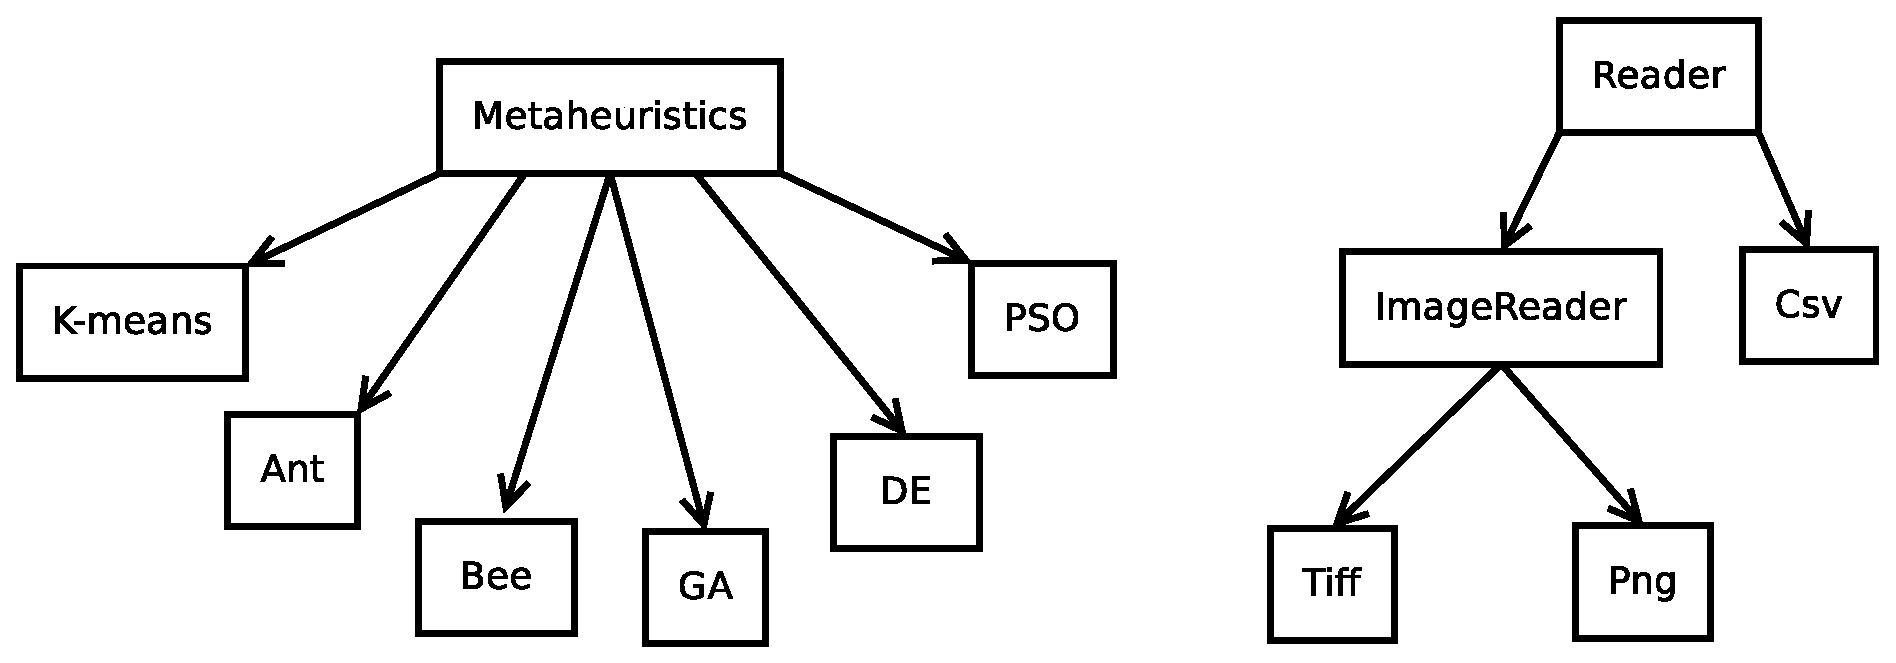
\includegraphics[scale=0.35]{figures/clases.eps}
\caption{Dise\~no de clases}
\label{fig:jclases}
\end{figure}

Donde Metaheuristics es una clase abstracta, que posee las m\'etodos que seran
usados por las diversas metaheur\'isticas hijas. En especial tienen dos 
importantes: initialize y run. El primero se va a encargar de inicializar el algoritmo
para que luego sea ejecutado. Por ejemplo en el gen\'etico inicializa aleatoriamente
las soluciones. Y el run es en s\'i el que va a ejecutar el algoritmo haciendo 
uso de los par\'ametros y variables ya inicilizadas.

Por el otro lado Reader tambi\'en
es una clase abstracta y es la que se encarga de definir lo m\'etodos que van a 
tener sus descendientes a la hora de leer un archivo, que se implement\'o para 
tres tipos: csv, png y tiff.

\section{M'aquina de prueba} \label{sect:testbed}

Todas las pruebas fueron realizadas con el computador cuyas caracter'isticas
aparecen en el cuadro \ref{tb:testbed}. La herramienta {\tt mhs} fue
compilada sobre esa m'aquina, exclusivamente con optimizaci'on gcc de nivel 3,
que es el nivel m\'as alto que posee gcc y aplica todas las mejoras
que este posee.

\begin{table}[htb]
\footnotesize
\begin{center}
\begin{tabular}{|>{\columncolor{lightgray}}c|c|}
\hline
CPU & Intel Core I5 650 \\
\hline
RAM & 6 GB \\
\hline
Distribuci'on & Ubuntu 11.04 x86\_64 bits \\
\hline
Kernel Linux & 2.6.38-8-generic \\
\hline
Versi'on gcc & 4.5.2 \\
\hline
\end{tabular}
\caption{Computador usado para las pruebas}
\label{tb:testbed}
\end{center}
\end{table}

\section{M\'etrica usada}

\section{K-means}

\'Este fue implementado tal cual como se explic\'o en \ref{sect:kmeans}. La
inicializaci\'on es totalmente aleatoria. Y la condici\'on de paradas
va a ser hasta que no se mejores un n\'umero de veces dado.

\section{Bee}

\section{Gen\'etico}

\section{DE}

\section{PSO}

\section{Hormiga}

Los resultados que se quieren evaluar est'an divididos en tres partes: 
Primero, es necesario verificar la calidad de estimaci'on del par'ametro
de Hurst usando los m'etodos implementados, segundo, es importante medir 
el tiempo necesario para cada estimaci'on y, por 'ultimo, es importante
comprobar si se pueden detectar ataques de denegaci'on de servicio mediante la
variaci'on del par'ametro y el uso del mecanismo de ventanas deslizantes.

La descripci'on del computador utilizado para ejecutar las pruebas se 
presenta en la secci'on \ref{sect:testbed}. Los archivos utilizados y los
resultados de la verificaci'on de la estimaci'on del par'ametro de Hurst y del
tiempo necesario para la estimaci'on se presentan en la secci'on
\ref{sect:validacion}. Estos resultandos muestran qu'e tan
preciso es la implementaci'on de los m'etodos y cu'anto tiempo en promedio
necesita la herramienta para estimar el valor del par'ametro de Hurst en una
ventana. 

\section{Validaci'on de los estimados} \label{sect:validacion}

Se ten'ia que probar que las implementaciones de los 3 m'etodos produc'ian
estimaciones razonables del par'ametro de Hurst para saber de antemano que tan
confiable podrian ser la estimaciones cuando se usasen junto con el mecanismo
de ventanas delizantes. Para la validaci'on de los m'etodos implementados se
probaron los mismos con datos producidos por el algoritmo de Paxson
\cite{Paxson95fastapproximation}.

El algoritmo de Paxson permite crear una serie de tiempo pseudo-aleatoria en
el dominio del tiempo de forma r'apida, y permite especificar el par'ametro de
Hurst a ser simulado y el n'umero de datos que debe tener la serie de tiempo
resultante, manteniendo la media en $0$ y la varianza en $1$, con valores
uniformemente distribuidos en el intervalo $[0,2\pi]$. Mediante el algoritmo
se puede simular un proceso estacionario autosimilar con dependencia de largo
alcance \cite{Paxson95fastapproximation}.

La implementaci'on del algoritmo de Paxson utilizada es la que viene en el 
paquete {\tt fArma} de {\tt R}. La validaci'on cont'o con 6 tama~nos diferentes
para la serie de tiempo $X_k$ generada por el algoritmo de Paxson. Estos 
tama~nos fueron $\{1024, 2048, 4096, 8192, 16384, 32768\}$. Por cada tama~no se
generaron 10 series de tiempo $X_k$ para cada uno de los 9 valores del
par'ametro de Hurst que se quer'ia simular. Estos valores fueron
$\{0.55, 0.60, 0.65, 0.70, 0.75, 0.80, 0.85, 0.90, 0.95 \}$. 
\begin{figure}[htb]
\centering
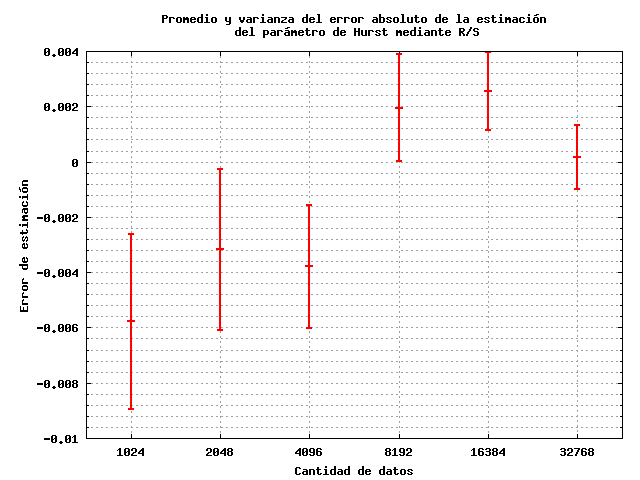
\includegraphics[scale=0.45,type=png,ext=.png,read=.png]{figures/abserror-rs}
\caption{Promedio y varianza del error absoluto de la estimaci'on del par'ametro
de Hurst para el m'etodo estad'istico R/S}
\label{fig:abserrrs}
\end{figure}

\begin{figure}[htb]
\centering
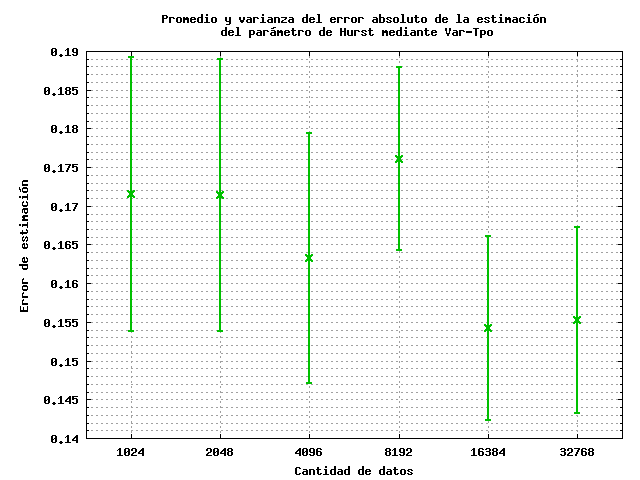
\includegraphics[scale=0.45,type=png,ext=.png,read=.png]{figures/abserror-var}
\caption{Promedio y varianza del error absoluto de la estimaci'on del par'ametro
de Hurst para el m'etodo de gr'aficas de varianza-tiempo}
\label{fig:abserrvar}
\end{figure}

\begin{figure}[htb]
\centering
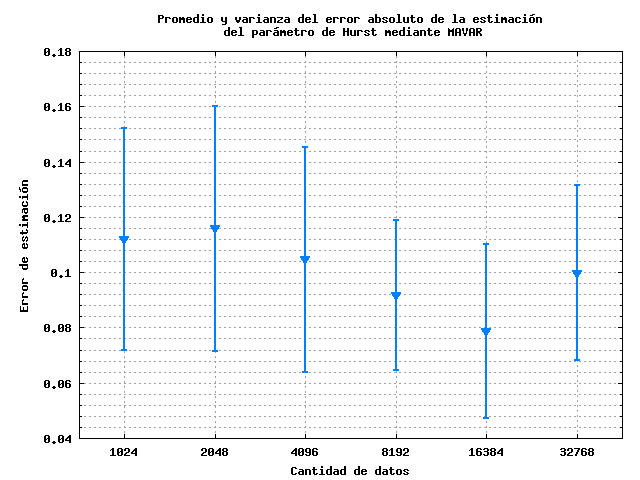
\includegraphics[scale=0.45,type=png,ext=.png,read=.png]{figures/abserror-mavar}
\caption{Promedio y varianza del error absoluto de la estimaci'on del par'ametro
de Hurst para el m'etodo de varianza modificada de Allan}
\label{fig:abserrmavar}
\end{figure}

\clearpage

\begin{figure}[htb]
\centering
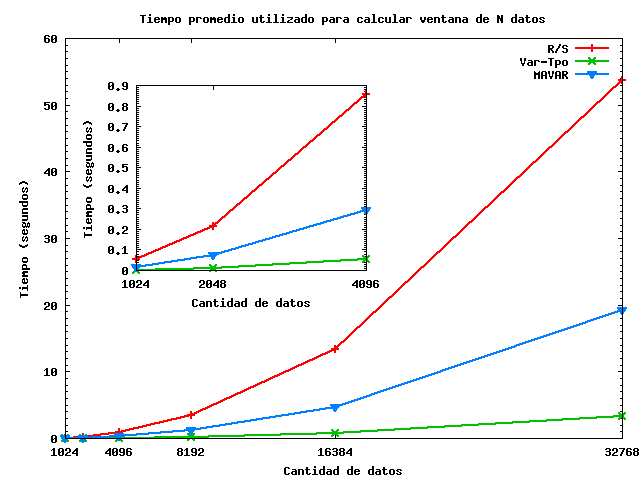
\includegraphics[scale=0.38,type=png,ext=.png,read=.png]{figures/time-n-plot}
\caption{Tiempo promedio utilizado para estimar una ventana de 1024 a 32768
datos para los m'etodos implementados}
\label{fig:tiempoventana}
\end{figure}

Observando las figuras \ref{fig:abserrrs}, \ref{fig:abserrvar} y
\ref{fig:abserrmavar}, lo que se puede evidenciar es que, en general, el
promedio del error absoluto de las estimaciones del par'ametro de Hurst de los
m'etodos mejoran y la varianza disminuye cuando se toman en cuenta un mayor
n'umero de datos para la ventana de estimaci'on. Sin embargo, para los
dos m'etodos que dependen de c'alculos con la varianza el promedio del error 
absoluto de la estimaci'on, incluso con el mayor n'umero de datos es mayor a
$0.1$. El m'etodo del estad'istico R/S es el m'etodo que se comporta mejora 
ya que tiene, en general, un error absoluto muy cerca a $0$ con una varianza
m'inima. 

De acuerdo a \cite{intelligentfuzzy} si queremos analizar los datos en tiempo
real para una red se tendr'ia que hacer una estimaci'on como m'inimo cada
segundo, por lo que una estimaci'on no puede tardar m'as de un segundo en
realizarse. Esto es seriamente limitante ya que cada m'etodo tiene un tiempo de
ejecuci'on muy diferente. Observando la figura \ref{fig:tiempoventana}, con
esta restricci'on la 'unica posibilidad que se tiene es limitar al m'etodo del
estad'istico R/S a $4096$ datos, al m'etodo de gr'aficas varianza-tiempo a
$16834$ datos y al m'etodo de varianza modificada de Allan a $4096$ datos. Dado
que para comparar los m'etodos es importante usar la misma cantidad de datos,
decidimos trabajar con $4096$ datos. El limitar el n'umero de datos va a
afectar la estimaci'on del par'ametro de Hurst directamente como se muestra en
las figuras \ref{fig:abserrrs}, \ref{fig:abserrvar} y \ref{fig:abserrmavar}. 

A pesar de estos problemas, seguimos adelante con el proyecto porque no
queremos una sola estimaci'on puntual y precisa de la traza, sino detectar su
variaci'on, por lo que optamos por un buen balance entre el tiempo de
ejecuci'on y el n'umero de datos a utilizar \cite{intelligentfuzzy}.



\chapter{Análisis de resultados}
\label{chap:analisis}

\section{Análisis de los resultados obtenidos con \emph{Lenna}}\label{sect:arimg}

    A continuación, se presenta un análisis comparativo entre todas las
metaheurísticas hibridas implementadas (\emph{GAH}, \emph{NPSOH}, \emph{WPSOH},
\emph{NDEH}, \emph{SDEH}, \emph{BeeH} y \emph{AntH}) y el algoritmo determinista
\emph{K-means}. Las metaheurísticas híbridas fueron elegidas para este análisis
por presentar mejor calidad en sus soluciones finales que las metaheurísticas no
híbridas (véase el apéndice \ref{apendicec}).

    Los datos utilizados provienen de los resultados obtenidos con el mejor
conjunto de valores encontrado para cada metaheurística con la imagen
\textbf{Lenna} (ver sección \ref{sect:impresultados} y apéndice \ref{apendicea}).

\subsection{Comparación por calidad de solución final: índice $DB$}\label{analisis:db}

    Como se mencionó en la sección \ref{sect:tval}, el índice $DB$ mide la
calidad de una partición en función de las distancias \emph{intra-cluster} e
\emph{inter-cluster}. Mientras menor sea el valor de este índice, se tiene mejor
calidad de partición.

\subsubsection{Prueba de diferencia de medias}\label{analisis:db_mean_hip}

    Para determinar diferencias en la calidad de las soluciones finales de los
algoritmos implementados y elegir al mejor de todos, se realizó una prueba de
hipótesis de diferencia de medias para el índice $DB$. Se debe probar para
cada par de algoritmos $i, j \in Algorithms \land i \neq j$ alguna de las
siguientes hipótesis:
\begin{itemize}
    \item \emph{Hipótesis nula}: $\bar{X}_i - \bar{X}_j = 0$
    \item \emph{Hipótesis altenativa}: $\bar{X}_i - \bar{X}_j \neq 0$
\end{itemize}
donde
\begin{itemize}
    \item $\bar{X}_i$ es la media de las observaciones del valor del índice $DB$
          para el algoritmo $i$.
    \item $Algorithms$ es el conjunto de grupos a estudiar. Está conformado por
los algoritmos implementados: \{\emph{K-means}, \emph{GAH}, \emph{NPSOH},
\emph{WPSOH}, \emph{NDEH}, \emph{SDEH}, \emph{BeeH}, \emph{AntH}\}.
\end{itemize}

\subsubsection{Prueba de diferencia de varianzas}\label{analisis:db_var_hip}

    Para determinar el estadístico de la prueba descrita en la sección
anterior (ver sección \ref{analisis:db_mean_hip}) es necesario saber si las
observaciones de los valores del índice $DB$ de los diferentes algoritmos
presentan homocedasticidad o heterocedasticidad (igual o diferente varianza
respectivamente). Fue elegida la prueba de \emph{Levene} \cite{Levene_Test}
debido a que permite la comparación de multiples grupos al mismo tiempo. Para
esta prueba se debe probar alguna de las siguientes hipótesis:
\begin{itemize}
    \item \emph{Hipótesis nula}: $\sigma_1 = \sigma_2 = \cdots = \sigma_i = \cdots = \sigma_n$
    \item \emph{Hipótesis alternativa}: al menos una de las varianzas es diferente.
\end{itemize}
donde $\sigma_i$ es la varianza poblacional del índice $DB$ para el algoritmo
$i$, $\forall i \in Algorithms$.

    El estadístico de la prueba de \emph{Levene} es el siguiente\cite{Levene_Test}:
\begin{equation}\label{levene_est}
    W = \displaystyle\frac{(N-k) \cdot \displaystyle\sum_{i = 1}^k N_i \cdot (Z_{i\cdot} - Z_{\cdot\cdot})^2}{(k - 1) \cdot \displaystyle\sum_{i = 1}^k \sum_{j = 1}^{N_i} (Z_{ij} - Z_{i\cdot})^2} \sim F_{\alpha, k - 1, N - k}
\end{equation}
donde
\begin{itemize}
    \item $k$ es la cantidad de grupos. Para efectos de esta prueba, es la
          cardinalidad del conjunto $Algorithms$.
    \item $N_i$ es el tamaño de la muestra para el algoritmo $i$.
    \item $N = \displaystyle\sum_{i \in Algorithms} N_i$
    \item $Y_{ij}$ es el $j$-ésimo valor de la muestra del algoritmo $i$.
    \item $Z_{ij} = |Y_{ij} - \tilde{Y}_i|$, donde $\tilde{Y}_i$
es la mediana de los valores de la muestra del algoritmo $i$.
    \item $Z_{\cdot\cdot} = \displaystyle\frac{1}{N} \displaystyle\sum_{i = 1}^k \sum_{j = 1}^{N_i} Z_{ij}$ es la media de todos los $Z_{ij}$.
    \item $Z_{i\cdot} = \displaystyle\sum_{j = 1}^{N_i} Z_{ij}$ es
la media del $Z_{ij}$ para el algoritmo $i$.
\end{itemize}

    Como se puede observar en el Resultado \ref{r_db_var_img} se rechaza la hipótesis
nula con un nivel de significancia menor a 5 \% (\emph{p-valor} $ = 6.025 \cdot 10^{-7}$).
Esto significa que existe una diferencia entre las varianzas de las muestras
del índice $DB$ de los algoritmos pertenecientes al conjunto $Algorithms$.
\textbf{Por lo tanto, las diferentes muestras presentan heterocedasticidad para
el índice $DB$}.

\begin{lstlisting}[float=h!, caption={Diferencia de Varianza: Índice \emph{DB}}, label=r_db_var_img]
> leveneTest(db, name)
Levene's Test for Homogeneity of Variance (center = median)
       Df F value    Pr(>F)    
group   7  6.4483 6.025e-07 ***
      231                      
---
Signif. codes:  0 '***' 0.001 '**' 0.01 '*' 0.05 '.' 0.1 ' ' 1 
\end{lstlisting}

\subsubsection{Intervalo de confianza de la prueba de diferencia de medias}\label{analisis:db_mean_est}

    En la sección anterior (ver sección \ref{analisis:db_var_hip}), se demostró
que las varianzas de las muestras del índice $DB$ de los algoritmos pertenecientes
al conjunto $Algorithms$ son diferentes. Por lo tanto, el estadístico de la prueba
de hipótesis descrita en la sección \ref{analisis:db_mean_hip} no debe ser
sensible a la varianza.

    Sobre los resultados se aplicó la prueba de \emph{Dunnett-Tukey-Kramer},
también llamada prueba \emph{T3} de \emph{Dunnett}, y fue elegida ya que
\cite{DTK_Test}:
\begin{itemize}
    \item No requiere que las varianzas de las muestras de los diferentes grupos
sean iguales.
    \item Permite la comparación de cada grupo con los demás sin aumentar la
probabilidad de cometer un error tipo I\footnote{Probabilidad de tener falsos
positivos}.
\end{itemize}

    El intervalo de confianza para la diferencia de medias de una prueba
\emph{T3} es el siguiente:
\begin{equation}\label{dtk_inter}
    \bar{X}_i - \bar{X}_j \pm q_{\alpha, k^{*}, \nu} \cdot \sqrt{\displaystyle\frac{S_{i}^2}{n_i} + \displaystyle\frac{S_{j}^2}{n_j}}
\end{equation}
donde
\begin{itemize}
    \item $\alpha$ es el nivel de confianza de la prueba.
    \item $\bar{X}_i - \bar{X}_j$ es la diferencia de medias del grupo $i$ con
el grupo $j$.
    \item $q$ es la distribución \emph{Studentized Range}.
    \item $i, j \in Algorithms$.
    \item $S_i$ es la varianza muestral del grupo $i$.
    \item $n_i$ es el tamaño de la muestra del grupo $i$.
    \item $k$ es la cantidad de grupos. Para efectos de esta prueba, es la
          cardinalidad del conjunto $Algorithms$.
    \item $k^{*}$ y $\nu$ son los grados de libertad del estadístico de la prueba:
          \begin{equation}
                k^{*} = \displaystyle\frac{k (k - 1)}{2}
          \end{equation}
          \begin{equation}\label{eq: nu}
            \nu = \displaystyle\frac{\left(\displaystyle\frac{S_{i}^2}{n_i} + \displaystyle\frac{S_{j}^2}{n_j}\right)^2}{\left(\displaystyle\frac{S_{i}^2}{n_i}\right)^2 \displaystyle\frac{1}{n_i - 1} + \left(\displaystyle\frac{S_{j}^2}{n_j}\right)^2 \displaystyle\frac{1}{n_j - 1}}
          \end{equation}
\end{itemize}

    En la figura \subref{fig:comp_inter} se pueden observar los intervalos de
confianza de la prueba \emph{T3} para el índice $DB$ de cada algoritmo comparado
con los demás. Los intervalos en rojo indican que existe una diferencia de calidad
de las soluciones finales de los algoritmos comparados con un nivel de significancia
de 5 \%. Por otro lado, los intervalos en negro indican que no existe una diferencia
de la calidad de las soluciones de los algoritmos comparados con un nivel de 
significancia de 5 \%. Por lo tanto, se puede concluir:
\begin{itemize}
    \item Los algoritmos \emph{K-means}, \emph{NPSOH}, \emph{WPSOH}, \emph{NDEH}
          y \emph{SDEH} tienen soluciones finales con calidad similar.
    \item Las metaheurísticas \emph{GAH} y \emph{BeeH} tienen soluciones finales
          con calidad similar y diferentes las de los demás algoritmos
          comparados.
    \item La calidad de las soluciones finales de la metaheurística \emph{AntH}
          es diferente a las calidades de las soluciones finales de los demás
          algoritmos.
\end{itemize}

    Tomando en cuenta el análisis anterior y el diagrama de cajas presentado en
la figura \subref{fig:comp_db}, se concluye:
\begin{itemize}
    \item Las metaheurísticas \emph{GAH} y \emph{BeeH} reportan los valores del
índice $DB$ promedio más bajo de todos los algoritmos comparados y, por lo tanto,
sus soluciones finales tienen mayor calidad que las de los demás algoritmos
implementados.
    \item La metaheurística \emph{AntH} reporta el valor del índice $DB$ promedio
más alto y, por lo tanto, sus soluciones finales tienen menor calidad que las de
los demás algoritmos implementados. Este comportamiento se puede observar con
claridad en en la figura \subref{fig:lennaant}, donde la imagen resultante
es difusa.
\end{itemize}

    \textbf{Así que las metaheurísticas cuyas soluciones finales tienen la mejor
calidad con respecto a las de los algoritmo implementados son \emph{GAH} y
\emph{BeeH}, ya que tienen los valores de índice $DB$ estadísticamente más bajos
(ver figuras \subref{fig:comp_db} y \subref{fig:comp_inter}).}

\begin{figure}[h!]
  \centering
  \subfloat[\emph{Diagramas de cajas del índice $DB$}]{\label{fig:comp_db}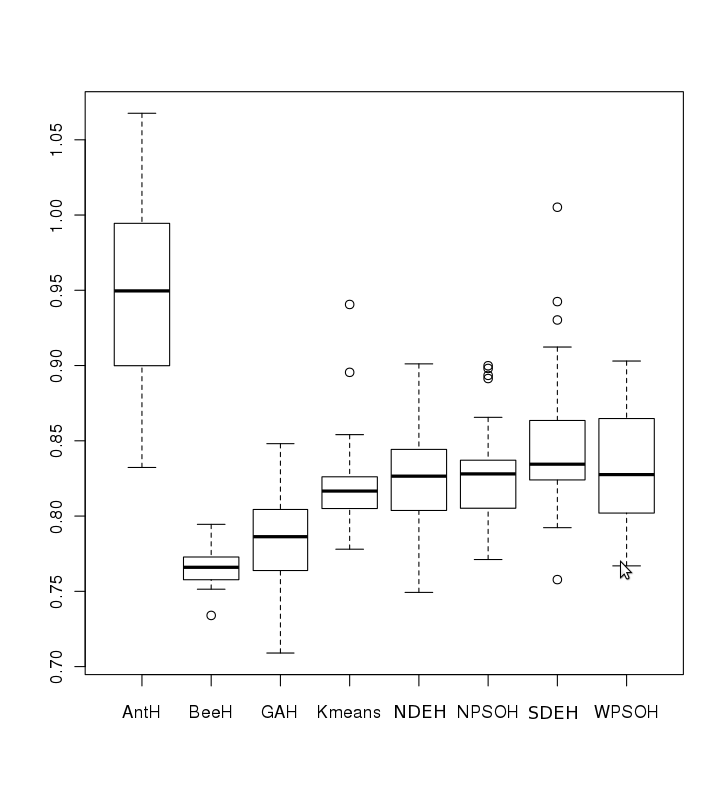
\includegraphics[width=0.6\textwidth]{figures/comp_db.png}}\\
  \subfloat[\emph{Intervalos de confianza del índice $DB$}]{\label{fig:comp_inter}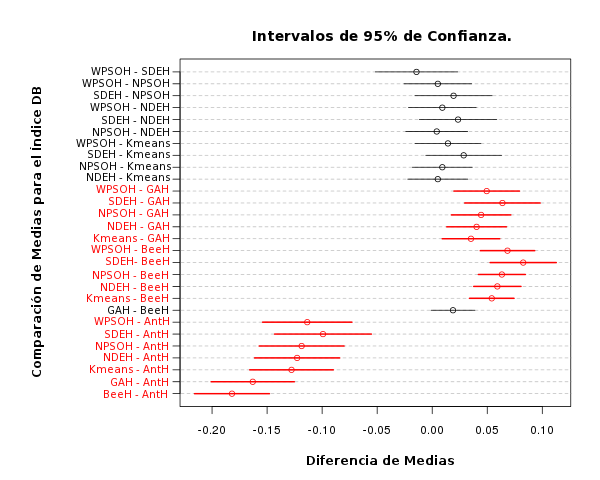
\includegraphics[width=0.6\textwidth]{figures/best_img_db.png}}
  \caption{Comparación del índice $DB$ para \textbf{Lenna}}
  \label{fig:alg_comp_lenna}
\end{figure}

\begin{figure}[h!]
  \centering
  \subfloat[\emph{AntH}]{\label{fig:lennaant}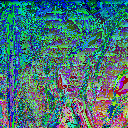
\includegraphics{figures/antlenna.png}} \qquad
  \subfloat[\emph{BeeH}]{\label{fig:lennabee}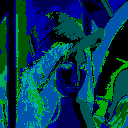
\includegraphics{figures/beelenna.png}} \qquad
  \subfloat[\emph{NDEH}]{\label{fig:lennande}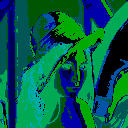
\includegraphics{figures/ndelenna.png}} \\
  \subfloat[\emph{GAH}]{\label{fig:lennaga}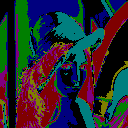
\includegraphics{figures/galenna.png}} \qquad
  \subfloat[\emph{K-means}]{\label{fig:lennakmeans}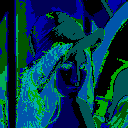
\includegraphics{figures/kmeanslenna.png}} \qquad
  \subfloat[\emph{NPSOH}]{\label{fig:lennapso}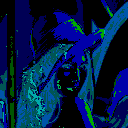
\includegraphics{figures/npsolenna.png}} \\
  \subfloat[\emph{SDEH}]{\label{fig:lennasde}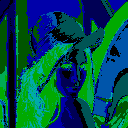
\includegraphics{figures/sdelenna.png}} \qquad
  \subfloat[\emph{WPSOH}]{\label{fig:lennawpso}
\includegraphics{figures/wpsolenna.png}} \qquad
  \subfloat[Original]{\label{fig:lennaoriginal}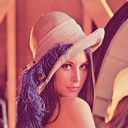
\includegraphics{figures/lenamini.png}} 
  \caption{Mejores soluciones encontradas para \textbf{Lenna}}
  \label{fig:lennaresults}
\end{figure}

\subsection{Comparación por la calidad de solución final: cuantificación del error $J_e$}

    Como se mencionó en la sección \ref{sect:tval}, la cuantificación del error
$J_e$ mide la calidad de una partición en función de la dispersión dentro de los
clusters de la misma. Mientras menor sea el valor de este error, se tiene mejor
calidad de partición.

\subsubsection{Prueba de diferencia de medias}\label{analisis:je_mean_hip}

    Para corroborar los resultados obtenidos en la sección \ref{analisis:db}, se
realizó una prueba de hipótesis de diferencia de medias para la cuantificación
del error $J_e$. Se debe probar para cada par de algoritmos $i, j \in Algorithms
\land i \neq j$ alguna de las siguientes hipótesis:
\begin{itemize}
    \item \emph{Hipótesis nula}: $\bar{X}_i - \bar{X}_j = 0$
    \item \emph{Hipótesis altenativa}: $\bar{X}_i - \bar{X}_j \neq 0$
\end{itemize}
\newpage
donde
\begin{itemize}
    \item $\bar{X}_i$ es la media de las observaciones del valor del error $J_e$
          para el algoritmo $i$.
    \item $Algorithms$ es el conjunto de grupos a estudiar (ver sección
          \ref{analisis:db_mean_hip}).
\end{itemize}

\subsubsection{Prueba de diferencia de varianzas}\label{analisis:je_var_hip}

    Para determinar el estadístico de la prueba descrita en la sección
anterior (ver sección \ref{analisis:je_mean_hip}) es necesario saber si las
observaciones de los valores del error $J_e$ de los di\-fe\-ren\-tes algoritmos
presentan homocedasticidad o heterocedasticidad (igual o diferente varianza
respectivamente). Al igual que en la sección \ref{analisis:db_var_hip}, fue
elegida la prueba de \emph{Levene} \cite{Levene_Test} debido a que permite la
comparación de varianzas de multiples grupos al mismo tiempo. Para esta prueba
se debe probar alguna de las siguientes hipótesis:
\begin{itemize}
    \item \emph{Hipótesis nula}: $\sigma_1 = \sigma_2 = \cdots = \sigma_i = \cdots = \sigma_n$
    \item \emph{Hipótesis alternativa}: al menos una de las varianzas es diferente.
\end{itemize}
donde $\sigma_i$ es la varianza poblacional del error $J_e$ para el algoritmo
$i \in Algorithms$. El estadístico de la prueba de \emph{Levene} está definido
por la ecuación (\ref{levene_est}).

    Como se puede observar en el Resultado \ref{r_je_var_img} se rechaza la hipótesis
nula con un nivel de significancia menor a 5 \% (\emph{p-valor} $ = 3.116 \cdot 10^{-5}$).
Esto significa que existe una diferencia entre las varianzas del error $J_e$
de las muestras de los algoritmos pertenecientes al conjunto $Algorithms$.
\textbf{Por lo tanto, las diferentes muestras presentan heterocedasticidad para
el error $J_e$}.

\begin{lstlisting}[float=h!, caption={Diferencia de Varianza: Cuantificación del error Je}, label=r_je_var_img]
> leveneTest(je, name)
Levene's Test for Homogeneity of Variance (center = median)
       Df F value    Pr(>F)    
group   7  4.9485 3.116e-05 ***
      231                      
---
Signif. codes:  0 '***' 0.001 '**' 0.01 '*' 0.05 '.' 0.1 ' ' 1 
\end{lstlisting}

\subsubsection{Intervalo de confianza de la prueba de diferencia de medias}\label{analisis:je_mean_est}

    En la sección anterior (ver sección \ref{analisis:je_var_hip}), se demostró
que las varianzas de las muestras del error $J_e$ de los algoritmos pertenecientes
al conjunto $Algorithms$ son diferentes. Por lo tanto, el estadístico de la
prueba de hipótesis descrita en la sección \label{analisis:je_mean_hip} no debe
ser sensible a la varianza.

    Sobre los resultados, se aplicó la prueba de \emph{Dunnett-Tukey-Kramer}, también
aplicada sobre las observaciones del índice $DB$ de los diferentes algoritmos
(ver sección \ref{analisis:db_mean_est}).

    En la figura \subref{fig:comp_inter_je}, se pueden observar los intervalos de
confianza de la prueba \emph{T3} para el error $J_e$ de cada algoritmo con los
demás. Los intervalos en rojo indican que existe una diferencia de calidad de las
soluciones finales de los algoritmos comparados con un nivel de significancia de
5 \%. Por otro lado, los intervalos en negro indican que no existe una diferencia
de la calidad de las soluciones de los algoritmos comparados con un nivel de 
significancia de 5 \%.

    De acuerdo a los intervalos de confianza mostrados en la figura
\subref{fig:comp_inter_je} y el diagrama de cajas que aparece en la figura
\subref{fig:comp_je}, se puede concluir que el mejor algoritmo es la
metaheurística \emph{AntH} ya que, en promedio, es diferente a los demás algoritmos
y su error $J_e$ es el más bajo. Sin embargo, esta es la única metaheurística
implementada que no logra definir de manera correcta los clusters de los archivos
de datos probados (\textbf{Lenna} e \textbf{Iris}), como se puede observar la
figura \subref{fig:lennaant}, donde la imagen resultante es difusa.

    El error $J_e$ es bajo para la metaheurística \emph{AntH} ya que ésta no
termina de agrupar los datos, dejando una gran cantidad de patrones dispersos en
clusters pequeños. Esto hace que la cuantificación del error $J_e$ sea ineficaz
para evaluar la verdadera calidad de la partición.

    \textbf{Se puede concluir entonces que el índice $DB$ es más confiable para
medir la calidad de una partición que la cuantificación del error $J_e$.}

\begin{figure}[h!]
  \centering
  \subfloat[\emph{Diagramas de cajas del error $J_e$}]{\label{fig:comp_je}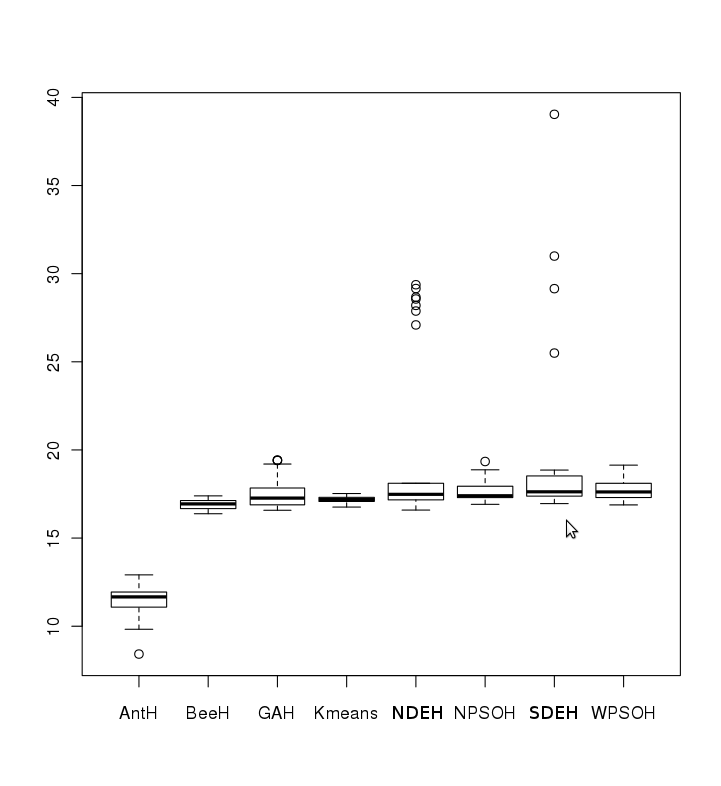
\includegraphics[width=0.6\textwidth]{figures/comp_je.png}}\\
  \subfloat[\emph{Intervalos de confianza del error $J_e$}]{\label{fig:comp_inter_je}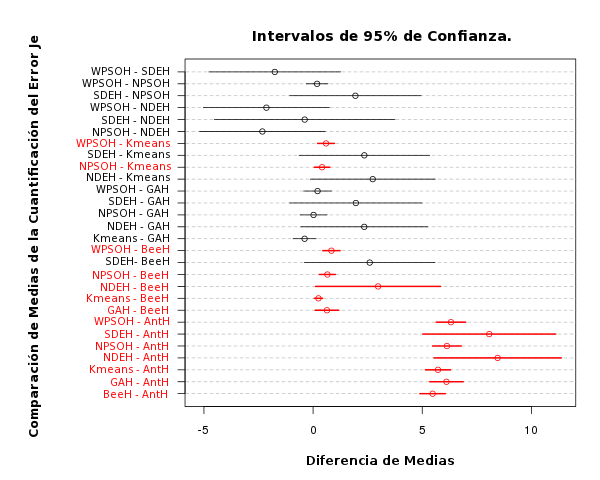
\includegraphics[width=0.6\textwidth]{figures/best_img_je.png}}
  \caption{Comparación del error $J_e$ para \textbf{Lenna}}
  \label{fig:alg_comp_lenna_je}
\end{figure}

\subsection{Comparación de \emph{GAH} y \emph{BeeH} en rendimiento}

    En la sección \ref{analisis:db}, se demostró que las metaheurísticas con 
mejor calidad en sus soluciones finales son \emph{GAH} y \emph{BeeH}. Sin
embargo, estas soluciones son estadísticamente similares, como se demostró en la
sección \ref{analisis:db_mean_est}, y por esto es necesario diferenciarlas
en rendimiento.

    Se utilizó la cantidad de evaluaciones de la función de \emph{fitness}
para comparar a las metaheurísticas \emph{GAH} y \emph{BeeH} porque es una
medida más justa que el tiempo de ejecución. La función de \emph{fitness} es la
función más costosa en tiempo de una metaheurística y la cantidad de veces que es
evaluada durante la ejecución es una cota inferior del tiempo total que pueda
tardar en ejecutarse. Esta medida es independiente del equipo y realmente
refleja el rendimiento de una metaheurística. Como ambas metaheurísticas usan la
misma función de \emph{fitness} para evaluar la calidad de sus soluciones (ver
capítulo \ref{sect:impresultados}), se estudió la cantidad de evaluaciones que
hacen \emph{GAH} y \emph{BeeH} de la misma, para determinar diferencias en el
rendimiento de estos algoritmos (ver apéndice \ref{apendicea}).

\subsubsection{Prueba de diferencia de medias}\label{analisis:eval_mean_hip}

    Se realizó una prueba de hipótesis de diferencia de medias para la cantidad
de evaluaciones de la función de \emph{fitness} de las metaheurísticas \emph{GAH}
y \emph{BeeH}. Se debe probar alguna de las siguientes hipótesis:
\begin{itemize}
    \item \emph{Hipótesis nula}: $\bar{X}_{GAH} - \bar{X}_{BeeH} = 0$
    \item \emph{Hipótesis altenativa}: $\bar{X}_{GAH} - \bar{X}_{BeeH} \neq 0$
\end{itemize}
donde $\bar{X}_{GAH}$ y $\bar{X}_{BeeH}$ son las medias muestrales de la
cantidad de evaluaciones de la función de \emph{fitness} de las metaheurísticas
\emph{GAH} y \emph{BeeH} respectivamente.
\newpage
    Para esto se utilizó la prueba $t$ de \emph{Welch} \cite{AB_0} la cual fue
elegida por no ser sensible a la varianza de los datos. El estadístico de la
prueba es como sigue:

\begin{equation}
    t = \displaystyle\frac{\bar{X}_{GAH} - \bar{X}_{BeeH}}{\sqrt{\frac{S_{GAH}^2}{n_{GAH}} + \frac{S_{BeeH}^2}{n_{BeeH}}}} \sim t_{\nu}
\end{equation}
donde,
\begin{itemize}
    \item $S_{GAH}$ y $S_{BeeH}$ son las varianzas muestrales para \emph{GAH} y
\emph{BeeH} respectivamente.
    \item $n_{GAH}$ y $n_{BeeH}$ son los tamaños de las muestras de \emph{GAH} y
\emph{BeeH} respectivamente.
    \item $\nu$ son los grados de libertad del estadístico y viene dado por la
          ecuación (\ref{eq: nu}) (ver sección \ref{analisis:db_mean_est}).
\end{itemize}

    Como se puede observar en el Resultado \ref{ga_bee_eval_img}, existe una
diferencia en la cantidad de evaluaciones de la función de \emph{fitness} de
ambas metaheurísticas con un nivel de significancia menor a 5 \%
(\emph{p-valor} $= 7.621 \cdot 10^{-16}$). Como la media de la metaheurística \emph{GAH}
($\bar{X}_{GAH} = 35.2069$) es estadísticamente menor que la de \emph{BeeH}
($\bar{X}_{BeeH} = 342.3333$), \emph{GAH} tiene mejor rendimiento que \emph{BeeH}.
\textbf{Por lo tanto, \emph{GAH} es la mejor de las metaheurísticas implementadas
para resolución del problema de \emph{data-clustering} con imágenes.}

\begin{lstlisting}[float=h!, caption={Diferencia de Medias: Evaluaciones de la función de \emph{fitness}}, label=ga_bee_eval_img]
> t.test(eval ~ name)

    Welch Two Sample t-test

data:  eval by name 
t = 15.6604, df = 29.533, p-value = 7.621e-16
alternative hypothesis: true difference in means is not equal to 0 
95 percent confidence interval:
 267.0475 347.2053 
sample estimates:
mean in group BeeH  mean in group GAH 
          342.3333            35.2069
\end{lstlisting}

\subsection{Prueba de la entonación con la imagen sintética}

    Para probar que la entonación de los parámetros de cada metaheurística fue
exitosa, se utilizó la imagen sintética mostrada en la figura \ref{fig:Trivial}
de la sección \ref{datatest}. Esta imagen tiene 7 clusters (6 formas geométricas
y el fondo).

    Como se puede observar en la figura \ref{fig:trivialresults}, todos los
algoritmos logran encontrar los 7 clusters, exceptuando la metaheurística
\emph{AntH}. En la figura \subref{fig:trivialant}, se puede observar algo de
ruido alrededor de algunas de las formas geométricas (puntos de colores),
demostrando que la metaheurística \emph{AntH} fue incapaz de ubicar algunos
patrones (pixeles) en los clusters donde les correspondía.

\begin{figure}[h!]
  \centering
  \subfloat[\emph{AntH}]{\label{fig:trivialant}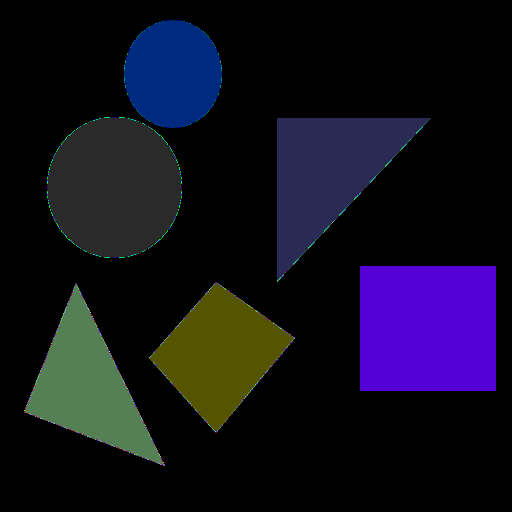
\includegraphics[scale=0.25]{figures/anttrivial.png}} \qquad
  \subfloat[\emph{BeeH}]{\label{fig:trivialbee}
\includegraphics[scale=0.25]{figures/beetrivial.png}} \qquad
  \subfloat[\emph{NDEH}]{\label{fig:trivialnde}
\includegraphics[scale=0.25]{figures/ndetrivial.png}} \\
  \subfloat[\emph{GAH}]{\label{fig:trivialga}
\includegraphics[scale=0.25]{figures/gatrivial.png}}  \qquad
  \subfloat[\emph{K-means}]{\label{fig:trivialkmeans}
\includegraphics[scale=0.25]{figures/kmeanstrivial.png}}  \qquad
  \subfloat[\emph{NPSOH}]{\label{fig:trivialpso}
\includegraphics[scale=0.25]{figures/npsotrivial.png}} \\
  \subfloat[\emph{SDEH}]{\label{fig:trivialsde}
\includegraphics[scale=0.25]{figures/sdetrivial.png}}  \qquad
  \subfloat[\emph{WPSOH}]{\label{fig:trivialwpso}
\includegraphics[scale=0.25]{figures/wpsotrivial.png}}  \qquad
  \subfloat[Original]{\label{fig:trivialoriginal}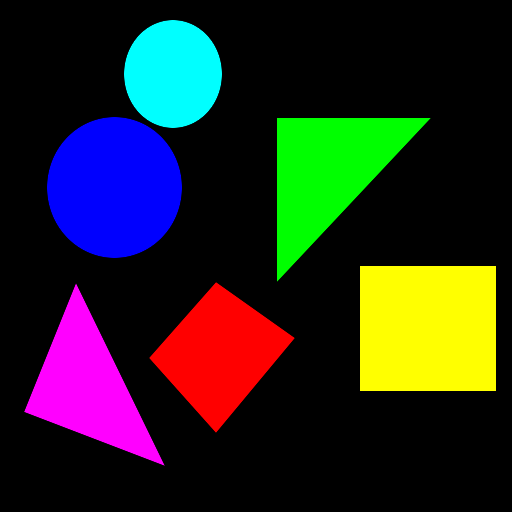
\includegraphics[scale=0.25]{figures/trivial.png}}
  \caption{Mejores soluciones encontradas para la imagen sintética}
  \label{fig:trivialresults}
\end{figure}

\section{Análisis de los resultados obtenidos con \emph{Iris}}\label{sect:arcsv}

    A continuación, se presenta un análisis comparativo (similar al hecho para la
imagen \textbf{Lenna}) entre todas las metaheurísticas hibridas implementadas
(\emph{GAH}, \emph{NPSOH}, \emph{WPSOH}, \emph{NDEH}, \emph{SDEH}, \emph{BeeH} y
\emph{AntH}) y el algoritmo determinista \emph{K-means}. Las metaheurísticas
híbridas fueron elegidas para este análisis por presentar mejor calidad en sus
soluciones finales que las metaheurísticas no híbridas (véase el apéndice
\ref{apendicec}).
    Los datos utilizados provienen de los resultados obtenidos con el mejor
conjunto de valores encontrado para cada metaheurística con el archivo de datos
numéricos \textbf{Iris} (ver sección \ref{sect:impresultados} y apéndice
\ref{apendicea}).

\subsubsection{Prueba de diferencia de medias}\label{analisis:db_mean_hip_csv}

    Para determinar diferencias en la calidad de las soluciones finales de los
algoritmos implementados y elegir al mejor de todos, se realizó una prueba de
hipótesis de diferencia de medias para el índice $DB$. Se debe probar para
cada par de algoritmos $i, j \in Algorithms \land i \neq j$ alguna de las
siguientes hipótesis:
\begin{itemize}
    \item \emph{Hipótesis nula}: $\bar{X}_i - \bar{X}_j = 0$
    \item \emph{Hipótesis altenativa}: $\bar{X}_i - \bar{X}_j \neq 0$
\end{itemize}
donde
\begin{itemize}
    \item $\bar{X}_i$ es la media de las observaciones del valor del índice $DB$
          para el algoritmo $i$.
    \item $Algorithms$ es el conjunto de grupos a estudiar (ver sección
          \ref{analisis:db_mean_hip}).
\end{itemize}

    Al igual que en la sección \ref{analisis:db_var_hip}, se realizó una prueba
de hipótesis de \emph{Levene} para determinar diferencia en las varianzas de los
datos. Como se puede observar en el Resultado \ref{r_db_var_csv} existe una diferencia
entre las varianzas del índice $DB$ de los diferentes grupos con un nivel de
significancia menor a 5 \% (\emph{p-valor} $ = 1.636 \cdot 10^{-15}$). \textbf{Por lo tanto,
las diferentes muestras presentan heterocedasticidad}.

\begin{lstlisting}[float=h!, caption={Diferencia de Varianza: Índice \emph{DB}}, label=r_db_var_csv]
> leveneTest(db, name)
Levene's Test for Homogeneity of Variance (center = median)
       Df F value    Pr(>F)    
group   7  14.692 1.636e-15 ***
      208                      
---
Signif. codes:  0 '***' 0.001 '**' 0.01 '*' 0.05 '.' 0.1 ' ' 1
\end{lstlisting}

    Debido a que las muestras presentan varianzas diferentes, se aplicó la prueba
\emph{T3} (ver sección \ref{analisis:db_mean_est}).

    En la figura \subref{fig:comp_inter_csv}, se puede observar los intervalos de
confianza de la prueba \emph{T3} para el índice $DB$ de cada algoritmo con los
demás. Los intervalos en rojo indican que existe una diferencia de calidad de las
soluciones finales de los algoritmos comparados con un nivel de significancia de
5 \%. Por otra lado, los intervalos en negro indican que no existe una diferencia
de la calidad de las soluciones de los algoritmos comparados con un nivel de 
significancia de 5 \%. Los resultados, son similares a los obtenidos en la
sección \ref{analisis:db_mean_est}. Sin embargo, se puede observar que para
\textbf{Iris}, las metaheurísticas \emph{GAH} y \emph{BeeH} presentan calidades
de soluciones finales estadísticamente diferentes. Al observar, además, el
diagrama de cajas presentado en la figura \subref{fig:comp_db_csv}, se puede
concluir que \textbf{\emph{GAH} es la metaheurística con mejor calidad en sus
soluciones finales con respecto a los demás algoritmos comparados, debido a que
su índice $DB$ es estadísticamente el más bajo.}

\begin{figure}[h!]
  \centering
  \subfloat[\emph{Diagramas de cajas del índice $DB$}]{\label{fig:comp_db_csv}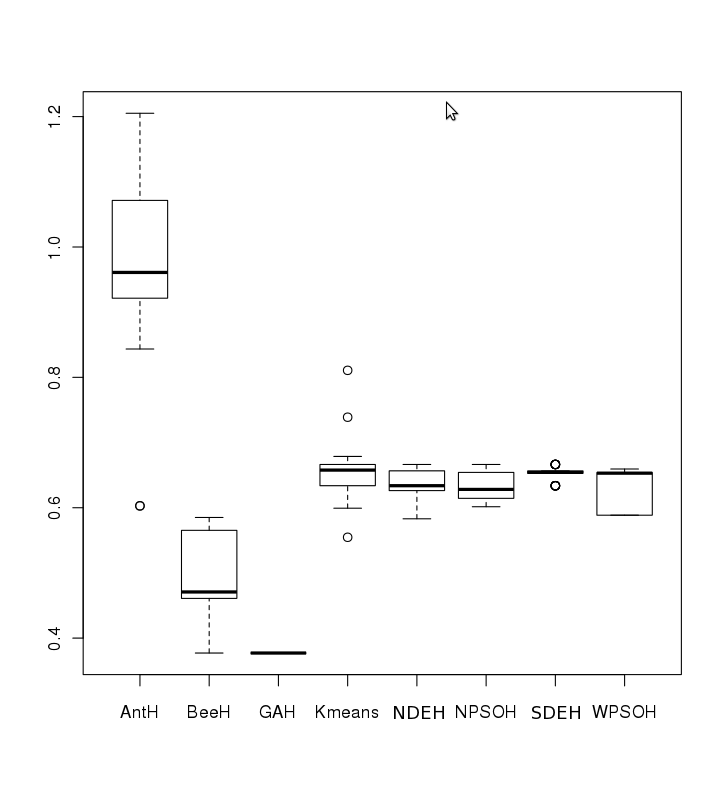
\includegraphics[width=0.6\textwidth]{figures/comp_db_csv.png}}\\
  \subfloat[\emph{Intervalos de confianza del índice $DB$}]{\label{fig:comp_inter_csv}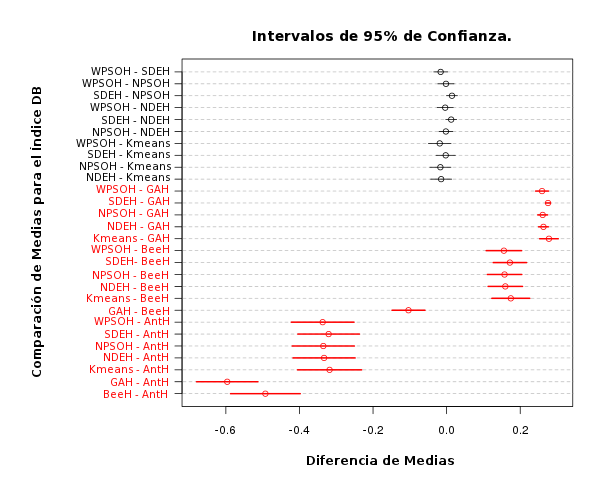
\includegraphics[width=0.6\textwidth]{figures/best_csv_db.png}}
  \caption{Comparación del índice $DB$ para \textbf{Iris}}
  \label{fig:alg_comp_lenna}
\end{figure}
\begin{comment}
\subsection{Imagen sintética}

    Una buena metaheurística sería capaz de particionar correctamente la imagen
sintética. Por lo tanto, fue usada para probar que se realizó una buena
entonación de los parámetros de cada metaheurística. Para más información de la
entonación de los parámetros, véase el apéndice \ref{apendicea}.

    En las figura \ref{fig:trivialresults} se pueden observar los resultados
de cada metaheurística para la imagen sintética. Todas éstas encontraron la
partición óptima para la imagen, exceptuando el \emph{Ant} que tiene ruido
(puntos de muchos colores) en los bordes de algunas de las formas geométricas.
Este ruido implica que la metaheurística \emph{Ant} fue incapaz de ubicar algunos
patrones (píxeles) en los clusters donde les correspondía.

\subsection{\textbf{Lenna}}

    A continuación, se presenta una tabla comparativa de los valores de los
índices de validez de las diferentes metaheurísticas implementadas. Los índices
reportados son los de las mejores soluciones de cada una de éstas para
\emph{Lenna}:

\begin{table}[H]
\footnotesize
\begin{center}
\begin{tabular}{|c|c|c|c|c|c|c|c|c|}
\hline
 & \emph{Ant} & \emph{Bee} & \emph{NDE} & \emph{GA} & \emph{K-means} & \emph{NPSO} & \emph{SDE} & \emph{WPSO} \\
\hline
{\bf DB} & 0.8323    & 0.734   & 0.7493 & 0.709   & 0.7814  & 0.7711  & 0.7578  & 0.7669 \\
\hline
$J_e$    & 11.2246   & 16.9922 & 16.589 & 19.4009 & 16.9164 & 17.3749 & 16.9559 & 16.9839 \\
\hline
{\bf EH} & 100160603 & 284     & 447    & 38      & 7       & 220     & 115     & 183     \\
\hline
\end{tabular}
\caption{Tabla comparativa de las metaheurísticas para {\bf Lenna}}
\label{tb:tableresimg}
\end{center}
\end{table}

    De la tabla \ref{tb:tableresimg} mostrada anteriormente, las gráficas
\ref{fig:alg_comp_lenna} y los resultados para \emph{Lenna} (figura
\ref{fig:lennaresults}), se puede apreciar:

\begin{itemize}
    \item A pesar que la metaheurística \emph{Ant} tiene el menor de los errores
    $J_e$, como se puede ver en la figura \subref{fig:comp_je}, sus soluciones no
    son buenas (ver figura \subref{fig:lennaant}) ya que se obtienen imágenes
    difusas. Esto hace que la cuantificación del error $J_e$ sea ineficaz para
    evaluar la verdadera calidad de la partición.

    El error $J_e$ es bajo para la metaheurística \emph{Ant} ya que ésta no
    termina de agrupar los datos, dejando una gran cantidad de patrones dispersos
    en clusters pequeños.

    \item En la tabla \ref{tb:tableresimg} y el diagrama de cajas \subref{fig:comp_db},
    se puede observar que los valores del índice $DB$ del \emph{Ant} son mayores
    que los de las demás metaheurísticas. Esto significa que es el peor de todos
    los algoritmos al no lograr construir particiones con distancia
     \emph{inter-cluster} alta y distancia \emph{intra-cluster} baja.

    \item En el diagrama \subref{fig:comp_je}, se puede observar un solapamiento
    en las cajas de todas las metaheurísticas, exceptuando el \emph{Ant}, indicando 
    que las medias del error $J_e$ son bastante parecidas entre ellas. Esto
    significa que los algoritmos están construyendo particiones con similar
    dispersión dentro de sus clusters.

    \item En el diagrama \subref{fig:comp_db}, se aprecia que las cajas de las
    metaheurísticas \emph{NDE}, \emph{NPSO}, \emph{SDE} y \emph{WPSO} se solapan,
    indicando que las medias de los valores del $DB$ son similares. Esto puede
    deberse a que comparten el mismo procedimiento que mantiene la cantidad de
    clusters fijos. Además, si comparamos los valores del $DB$ de estas
    metaheurísticas con los de \emph{K-means}, se puede ver que son similares,
    pero tienen mayor valor de \textbf{EH} (véase la tabla \ref{tb:tableresimg}).
    Esto nos permite inferir que estas metaheurísticas no son competitivas con el
    \emph{K-means}.

    \item Sólo las metaheurísticas \emph{Bee} y \emph{GA} muestran valores de
    $DB$ que superan, en promedio, los valores para el algoritmo determinista
    \emph{K-means} (véase diagrama \subref{fig:comp_db}), lo que las hacen ser
    las metaheurísticas de mejor calidad y rendimiento de las implementadas.

    \item En el diagrama \subref{fig:comp_db}, las cajas de los algoritmos
    \emph{Bee} y \emph{GA} se solapan. Esto significa que los valores promedio
    del índice $DB$ son similares y, por ende, ambos consiguen buenas soluciones
    finales por igual. Sin embargo, existen varias diferencias fundamentales
    entre estos dos algoritmos:
    \begin{itemize}
        \item El \emph{GA} no necesita saber de antemano la cantidad total de
        clusters, sino que sólo requiere conocer una cota superior. En cambio, 
        el \emph{Bee} necesita el número de clusters exacto para poder encontrar
        una buena solución.

        \item El \emph{GA} necesita una menor cantidad de evaluaciones promedio
        que el \emph{Bee} lo que la hace una metaheurística más rápida
        (véase diagrama \subref{fig:comp_eval}).
    \end{itemize}
\end{itemize}


\begin{figure}[H]
  \centering
  \subfloat[\emph{Índice $DB$}]{\label{fig:comp_db}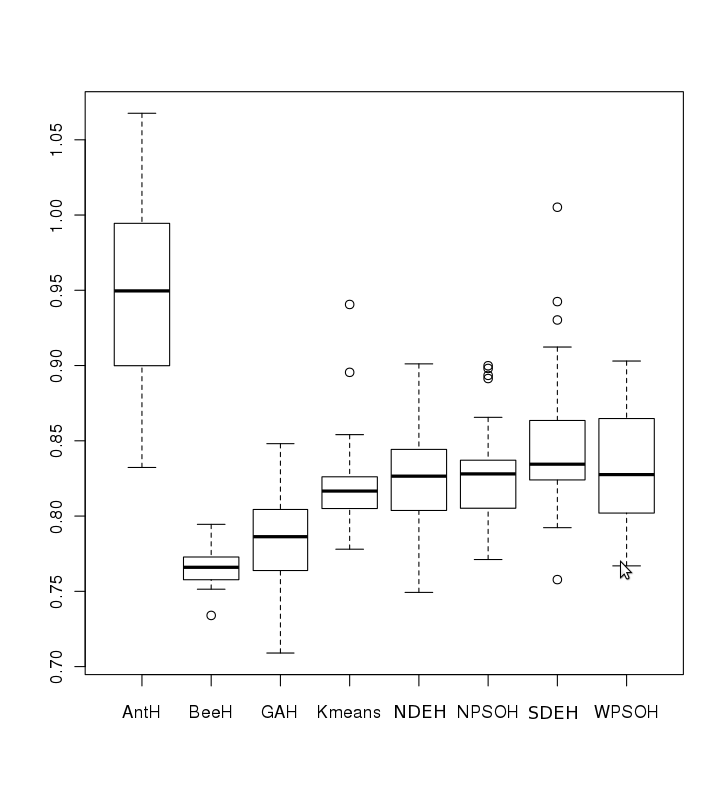
\includegraphics[width=0.5\textwidth]{figures/comp_db.png}}
  \subfloat[\emph{Cuantificación del error $J_e$}]{\label{fig:comp_je}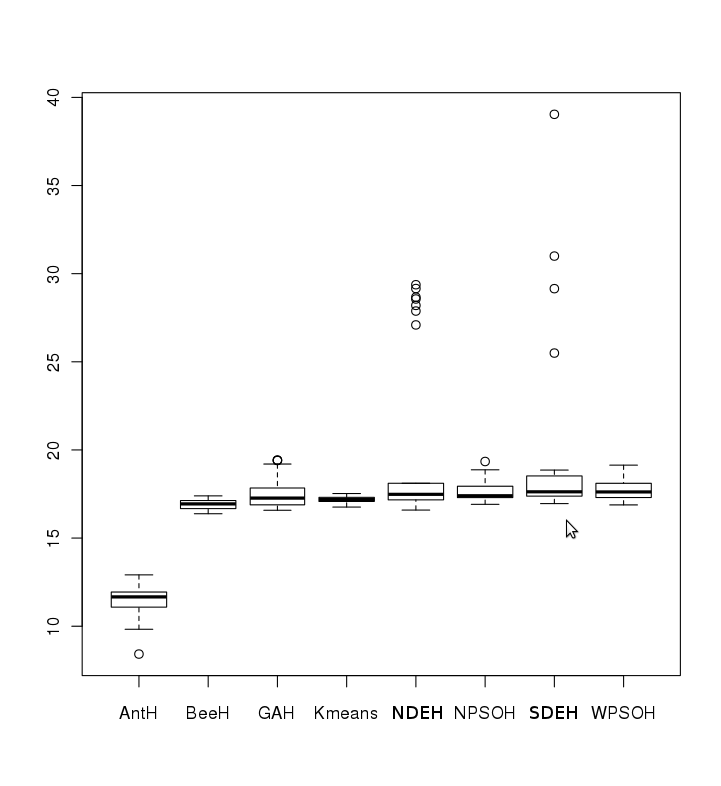
\includegraphics[width=0.5\textwidth]{figures/comp_je.png}}\\
  \subfloat[\emph{Cantidad de evaluaciones totales \textbf{EH}}]{\label{fig:comp_eval}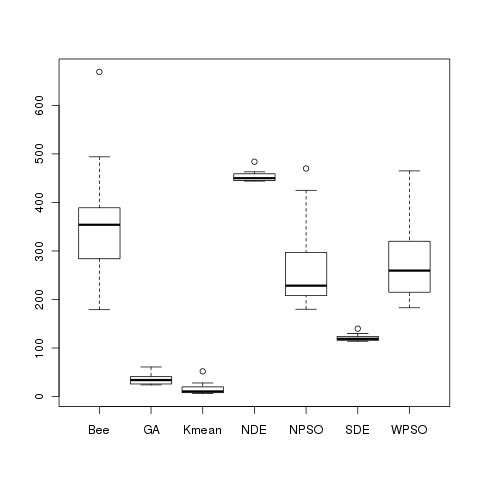
\includegraphics[width=0.5\textwidth]{figures/comp_eval.png}}
  \caption{Diagramas de cajas del $DB$, $J_e$ y \textbf{EH} para \textbf{Lenna}}
  \label{fig:alg_comp_lenna}
\end{figure}

\begin{figure}
  \centering
  \subfloat[\emph{Ant}]{\label{fig:trivialant}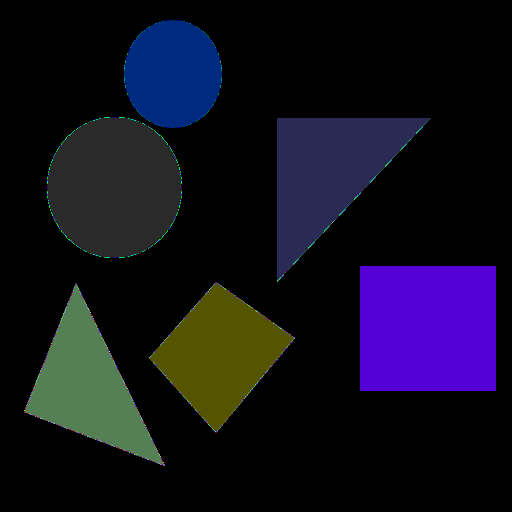
\includegraphics[scale=0.25]{figures/anttrivial.png}} \qquad
  \subfloat[\emph{Bee}]{\label{fig:trivialbee}
\includegraphics[scale=0.25]{figures/beetrivial.png}} \qquad
  \subfloat[\emph{NDE}]{\label{fig:trivialnde}
\includegraphics[scale=0.25]{figures/ndetrivial.png}} \\
  \subfloat[\emph{GA}]{\label{fig:trivialga}
\includegraphics[scale=0.25]{figures/gatrivial.png}}  \qquad
  \subfloat[\emph{K-means}]{\label{fig:trivialkmeans}
\includegraphics[scale=0.25]{figures/kmeanstrivial.png}}  \qquad
  \subfloat[\emph{NPSO}]{\label{fig:trivialpso}
\includegraphics[scale=0.25]{figures/npsotrivial.png}} \\
  \subfloat[\emph{SDE}]{\label{fig:trivialsde}
\includegraphics[scale=0.25]{figures/sdetrivial.png}}  \qquad
  \subfloat[\emph{WPSO}]{\label{fig:trivialwpso}
\includegraphics[scale=0.25]{figures/wpsotrivial.png}}  \qquad
  \subfloat[Original]{\label{fig:trivialoriginal}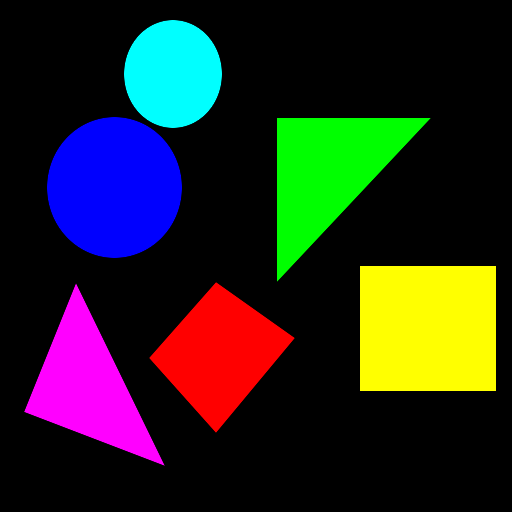
\includegraphics[scale=0.25]{figures/trivial.png}}
  \caption{Mejores soluciones encontradas para la imagen sintética}
  \label{fig:trivialresults}
\end{figure}

\begin{figure}
  \centering
  \subfloat[\emph{Ant}]{\label{fig:lennaant}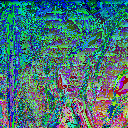
\includegraphics{figures/antlenna.png}} \qquad
  \subfloat[\emph{Bee}]{\label{fig:lennabee}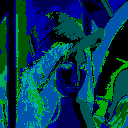
\includegraphics{figures/beelenna.png}} \qquad
  \subfloat[\emph{NDE}]{\label{fig:lennande}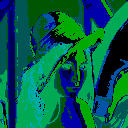
\includegraphics{figures/ndelenna.png}} \\
  \subfloat[\emph{GA}]{\label{fig:lennaga}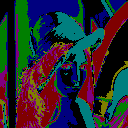
\includegraphics{figures/galenna.png}} \qquad
  \subfloat[\emph{K-means}]{\label{fig:lennakmeans}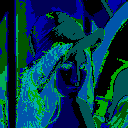
\includegraphics{figures/kmeanslenna.png}} \qquad
  \subfloat[\emph{NPSO}]{\label{fig:lennapso}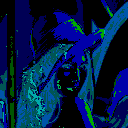
\includegraphics{figures/npsolenna.png}} \\
  \subfloat[\emph{SDE}]{\label{fig:lennasde}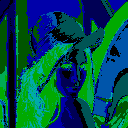
\includegraphics{figures/sdelenna.png}} \qquad
  \subfloat[\emph{WPSO}]{\label{fig:lennawpso}\includegraphics{figures/wpsolenna.png}} \qquad
  \subfloat[Original]{\label{fig:lennaoriginal}\includegraphics{figures/lenamini.png}} 
  \caption{Mejores soluciones encontradas para \textbf{Lenna}}
  \label{fig:lennaresults}
\end{figure}

\section{Resultados para \textbf{Iris}}\label{sect:arcsv}

    A continuación, se presenta una tabla comparativa de los valores de los
índices de validez las diferentes metaheurísticas implementadas. Los índices
reportados son los de las mejores soluciones de cada una de éstas para \emph{Iris}:

\begin{table}[h!]
\footnotesize
\begin{center}
\begin{tabular}{|c|c|c|c|c|c|c|c|c|}
\hline
 & \emph{Ant} & \emph{Bee} & \emph{NDE} & \emph{GA} & \emph{K-means} & \emph{NPSO} & \emph{SDE} & \emph{WPSO} \\
\hline
{\bf DB}  & 0.6029  & 0.3771 & 0.583  & 0.3771 & 0.599  & 0.6015 & 0.6338 & 0.5885 \\
\hline
$J_e$     & 0.4881  & 0.5029 & 0.6586 & 0.5029 & 0.6339 & 0.6807 & 0.625  & 0.6709 \\
\hline
{\bf EH}  & 1000163 & 304    & 170    & 47     & 5      & 130    & 171    & 45     \\
\hline
\end{tabular}
\caption{Tabla comparativa de las metaheurísticas para {\bf Iris}}
\label{tb:tablerescsv}
\end{center}
\end{table}

        De la tabla \ref{tb:tablerescsv} mostrada anteriormente y las gráficas
\ref{fig:alg_comp_iris}, se puede llegar a conclusiones similares a las
obtenidas para \textbf{Lenna}. Sin embargo, se pueden apreciar las siguientes
diferencias:
\begin{itemize}
    \item En el diagrama \subref{fig:comp_db_csv}, se puede observar que el
    \emph{GA} tiene mejores valores de índice $DB$, en promedio, que el \emph{Bee},
    No obstante, ambas metaheurísticas siguen superando a las demás.

    \item A diferencia de los resultados para \textbf{Lenna}, las distribuciones
    del error $J_e$ para el \emph{GA} y el \emph{Bee} superan a las de las
    demás metaheurísticas (véase el diagrama \subref{fig:comp_db_csv}).
\end{itemize}

\begin{figure}[H]
  \centering
  \subfloat[\emph{Índice $DB$}]{\label{fig:comp_db_csv}\includegraphics[width=0.5\textwidth]{figures/comp_db_csv.png}}
  \subfloat[\emph{Cuantificación del error $J_e$}]{\label{fig:comp_je_csv}\includegraphics[width=0.5\textwidth]{figures/comp_je_csv.png}}\\
  \subfloat[\emph{Cantidad de evaluaciones totales \textbf{EH}}]{\label{fig:comp_eval_csv}\includegraphics[width=0.5\textwidth]{figures/comp_eval_csv.png}}
  \caption{Diagramas de cajas del $DB$, $J_e$ y \textbf{EH} para \textbf{Iris}}
  \label{fig:alg_comp_iris}
\end{figure}

\end{comment}

% Conclusiones
\chapter{Conclusiones} \label{chap:conclusiones}

    En este capítulo, se presentan los hallazgos y contribuciones de este
proyecto y se dan algunas recomendaciones para futuros trabajos:
\begin{comment}
    Se evaluó el desempeño de los algoritmos \emph{K-means}, \emph{GAH},
\emph{NPSOH}, \emph{WPSOH}, \emph{NDEH}, \emph{SDEH}, \emph{BeeH}, \emph{AntH}.
Estos ocho algoritmos fueron comparados mediante el índice de validez $DB$ y la
cuantificación del error $J_e$ para determinar la calidad de sus soluciones
finales. Además, se comparó el rendimiento de las metaheurísticas \emph{GAH} y
\emph{BeeH} por medio de la cantidad de evaluaciones de su función de \emph{fitness}.
Así que, en función del análisis hecho en el capítulo anterior (ver capítulo \ref{chap:analisis}),
se puede concluir:
\end{comment}

\begin{itemize}
    \item Se llevó a cabo un estudio comparativo entre los algoritmos \emph{K-means},
          \emph{GAH}, \emph{NPSOH}, \emph{WPSOH}, \emph{NDEH}, \emph{SDEH},
          \emph{BeeH} y \emph{AntH} donde \emph{BeeH} y \emph{GAH} resultaron
          ser las mejores metaheurísticas.

    \item Se encontró que \emph{GAH} necesita probabilidades de mutación altas
          ($\geq 0.5$) para que sus soluciones finales sean de calidad.

    \item Se recomienda usar \emph{GAH} cuando no se tenga conocimiento a priori
          del número de clusters.

    \item El índice de validez $DB$ es más eficaz para medir la calidad de una
          partición que la cuantificación de error $J_e$. Esto se debe a que $J_e$
          se ve afectado por la cardinalidad de los clusters.

    \item Las soluciones finales de las metaheurísticas híbridas \emph{NPSOH},
          \emph{WPSOH}, \emph{NDEH}, \emph{SDEH} son similares en calidad. Esto
          puede deberse a que comparten procedimientos.

    \item El \emph{AntH} fue la peor metaheurística implementada. Este comportamiento
          se le atribuye a que no se logró realizar una implementación que
          reprodujera los resultados del artículo \cite{OuBa2007}.

    \item Las metaheurísticas híbridas arrojaron mejores resultados que sus
          contrapartes no híbridas.
          
\end{itemize}

\begin{comment}
\begin{itemize}

	\item El \emph{BeeH} y el \emph{GAH} resultaron ser las mejores metaheurísticas.
    Sin embargo, el \emph{GAH} consiguió soluciones finales con una calidad parecida
    a las del \emph{BeeH} utilizando menos evaluaciones de la función de
    \emph{fitness}.

	\item El \emph{GAH} es la única metaheurística que no requiere la cantidad
    de clusters lo cual es una ventaja cuando no se conoce \emph{a priori}.

	\item Tener una alta probabilidad de mutación ($\geq 0.5$) en el \emph{GAH}
	genera mejores resultados, indicando que el problema de \emph{data clustering}
    necesita grandes modificaciones en los vectores de centroides de sus
    individuos para obtener buenas soluciones.

    \item El índice de validez $DB$ es más eficaz para medir la calidad de una
    partición que la cuantificación del error $J_e$. Esto se debe a que el error
    $J_e$ sugería que la metaheurística \emph{AntH} era la mejor de todas las
    metaheurísticas implementadas. Sin embargo, resultados como los mostrados en
    las figuras \subref{fig:lennaant} y \subref{fig:trivialant}, donde se observa
    mucho ruido, demuestran lo contrario.
    

	\item Las metaheurísticas \emph{NDEH}, \emph{SDEH}, \emph{NPSOH} y \emph{WPSOH}
    comparten un procedimiento para mantener el número de clusters fijo y esto
	podría estar afectando su desempeño, haciendo que sus soluciones sean similares
    entre sí.

	\item El \emph{AntH} fue la peor metaheurística implementada. Este comportamiento
    puede tener su origen en que no se logró hacer una implementación que
    reprodujera los resultados reportados en el artículo base \cite{OuBa2007}.
    En este artículo, no habían suficientes detalles sobre la implementación
    de la memoria de las hormigas y esto pudo haber llevado a una implementación
    ineficiente de la metaheurística \emph{AntH}.
\end{itemize}

\end{comment}

	A partir de los resultados y conclusiones de este proyecto de grado, se pueden
dar las siguientes recomendaciones:

	Primero, es posible que los resultados de las metaheurísticas sean sensibles
a los conjuntos de datos a particionar. Es por esto que todas las metaheurísticas deberían ser probadas
con otros conjuntos de datos, además de \textbf{Lenna} e \textbf{Iris}, de modo
que se corrobore lo dicho en este proyecto de grado.

	Segundo, buscar un nuevo enfoque para la memoria del \emph{AntH}, de modo que
se puedan reproducir los resultados del artículo \cite{OuBa2007}. En este
artículo, no habían suficientes detalles sobre la misma y la implementación
realizada pudo haber afectado el desempeño de esta metaheurística.

	Por último, el procedimiento para mantener los clusters fijos que comparten
las metaheurísticas \emph{NDEH}, \emph{SDEH}, \emph{NPSOH} y \emph{WPSOH} pudo
haber afectado su desempeño. Buscar un nuevo enfoque para este procedimiento,
podría lograr una mejora en los resultados de estas metaheurísticas.


% Crea el glosario 
\printglossaries

% Establece las citas y bibliografia
\bibliographystyle{alpha.bst}
\bibliography{myrefs}

% Crea el apendice
\appendix
% Apendice
\chapter{Informaci'on adicional de {\tt d2Hgr}}

AQU\'I VA EL CONTENIDO DE LOS AP\'ENDICES.
%Puedes quitar esto(es opcional)
\vspace{5 mm}

Esta parte del ap'endice contiene el manual del usuario de la herramienta
implementada, la descripci'on de sus archivos y el c'odigo fuente de algunos
m'odulos de posible inter'es.

\section{Requerimientos de {\it software} y {\it hardware}}
\label{sect:hardsoftrequirements}

El programa resultante deber'ia poder ser utilizado sobre cualquier maquina 
con m'as de 32 MB libres de RAM. Aunque no hay limitaciones para el procesador
a usar, entre m'as nuevo el procesador y mayor n'umero de n'ucleos tenga, m'as
r'apido har'a los calculos la herramienta. En el caso de la memoria, entre 
m'as tenga disponible la herramienta, mayor cantidad de datos podr'a utilizar 
en los c'alculos.

\begin{itemize}
\item Para su compilaci'on, el programa requiere una versi'on actualizada de
gcc, el compilador {\tt C} GNU. Se ha utilizado varias versiones para su
compilaci'on por lo cualquier versi'on mayor a la $4.2$ deber'ia funcionar.
\item La liber'ia {\tt libpcap} es necesaria para darle las funcionalidades de
manipulaci'on de trazas {\tt tcpdump} al programa. A partir de la versi'on
$0.8$ se encuentran todas las funciones que utiliza el programa.
\item La compilaci'on de la herramienta se hace m'as f'acil con {\tt make},
programa GNU. Cualquier versi'on mayor a $3.6$ no deber'ia dar problemas.
\item El programa {\tt gnuplot} es indispensable para poder graficar los
resultados creados por el programa. La versi'on m'as utilizada durante su
desarrollo fue la $4.2$ por lo que es la que se recomienda.
\item La graficaci'on s'olo se puede hacer sobre un sistema operativo bajo el
est'andar POSIX\footnote{"Portable Operating System Interface [for Unix]" son
una familia de est'andares de llamadas al sistema operativo definidos por la
IEEE y especificados formalmente en el IEEE 1003. La gran mayor'ia de las
distribuciones GNU/Linux siguen los est'andares aunque no est'an
oficialmente certificados.} con la herramienta gnuplot instalada. Esto se debe
a una necesidad de la interfaz gnuplot en ANSI C que utiliza un ``pipe'' tipo
POSIX para comunicarse directamente con el programa gnuplot instalado en la
m'aquina. Sin embargo, dentro de las opciones del programa se puede pasar la
informaci'on obtenida en la estimaci'on a archivos de texto para su posterior
an'alisis.
\item La librer'ia pthreads da las funciones necesarias para utilizar hilos
de ejecuci'on en el programa.
\end{itemize}

\section{Ayuda de la l'inea de comando} \label{sect:ayuda}

La herramienta toma como par'ametro principal un archivo {\tt tcpdump} o un CSV
de una serie de tiempo pseudo-aleatoria generada con la herramienta R.
Aparte se puede escoger una velocidad de captura, una ventana, una ventana
deslizante, filtrar paquetes, delimitar corridas, correr con varios hilos de
ejecuci'on, adem'as de estimar el par'ametro de Hurst con los tres m'etodos
mencionados. Se puede tambi'en obtener el cambio del par'ametro de Hurst en el
tiempo o graficar la estimaci'on de una ventana en particular. La ayuda de la
l'inea de comando se muestra abajo:

\begin{alltt}
\label{verb:help}
Usage: ./d2Hgr -[f|g] file -[i|nrlvxmu] [OPTIONS]                               

Estimate and graph Hurst parameter calculations from a file.

   -f file   Specifies a tcpdump dump file.
   -g file   Specifies a CSV file with a simulated network traffic stream.
             This option cannot be used with the time based or tcpdump
             options since the stream is simulated and is static in it's
             definition.
   -i        Prints only the protocol statistic information available from the
             tcpdump file.
   -n        Tells the program if you wish to graph the packets per delta time
             graph. Affected by -p, -o, -d, -c, -b -e, -y flags.
   -r        Tells the program to calculate the Hurst parameter changes over
             time by use of the R/S statistic. Affected by -p, -o, -d, -c, -w,
             -s, -j, -t, -b, -e, -y flags.
   -l num    Tells the program to graph the Pox diagram that creates the Hurst
             data point for a given window number between 0 and Datapoints
             designated by num. Affected by -p, -o, -d, -c, -w, -s, -j, -b,
             -e, -y flags.
   -v        Tells the program to calculate the Hurst parameter changes over
             time by using the Variance-time plot technique. Affected by -p,
             -o, -d, -w, -s, -j, -t, -b, -e, -y flags.
   -x num    Tells the program to graph the Variance-time plot that estimates
             the Hurst parameter for a given window number designated by num.
             Affected by -p, -o, -d, -c, -w, -s, -j, -b, -e, -y flags.
   -m        Tells the program to calculate the Hurst parameter changes over
             time by use of the Modified Allan Variance. Affected by -p, -o,
             -d, -c, -w, -s, -j, -t, -b, -e, -y flags.
   -u num    Tells the program to graph the Modified Allan Variance that
             estimates the Hurst parameter for a given window number designated
             by num. Affected by -p, -o, -d, -c, -w, -s, -j, -t, -b, -e, -y
             flags.

 OPTIONS:
   -p proto  Specifies which protocol to be taken into account when doing
             calculations. Default is all.
             Implemented protocols are:
              ip tcp udp icmp sctp ftp ssh telnet smtp dns dhcp http pop3 ntp
              imap snmp ldap https smtps ldaps imaps pop3s nfs squid
   -o dir    Output directory for results. Default is current directory.
   -d        Tells the program if the results should be placed in text files
             for later use. This option doesn't graph. Useful for using this
             program where gnuplot is not available.
   -y        Tells the program to graph and print the resulting data files.
   -a        Tells the program not to graph or create data files.
   -c sec    Specify a packet capture speed. This makes the program not look
             for one. Example: 0.01 = 0.01 seconds.
   -w sec    Window time size. This makes the program not look for one.
             Example: 60 = 60 seconds.
   -s sec    Slide time size. This makes the program not look for one.
             Example: 1 = 1 seconds.
   -j num    Tells the program to use log base num for all the calculations of
             blocks for the R/S statistic, Variance-time plot and Modified Allan
             Variance. Default is 2.
   -t num    Does Hurst calculation using threads. If 0 is placed, then the
             default number of threads (4) is used.
   -b sec    Tells the program from which second in the time data to begin the
             calculation. Default is 0s.
   -e sec    Tells the program how many seconds after the beginning point to
             include in the calculation. Default is the whole tcpdump time.
   -k num    Average Hurst parameter change with which to try to detect attacks.
   -K num    Standard deviation of Hurst parameter change with which to detect
             attacks.
   -q num    Average Hurst parameter value with which to try to detect attacks.
   -Q num    Standard deviation of Hurst parameter value with which to detect
             attacks.
   -h        Print this help.
\end{alltt}

\section{Archivos del programa}

El programa de C llamado {\tt d2Hgr}, consiste de 18 archivos de c'odigo fuente
que incluye 9 archivos de cabecera. Los archivos contienen la siguiente
informaci'on:

\begin{itemize}
\item{\bf config.h}: Cabecera de funciones para parsear las opciones de linea
de comando.
\item{\bf config.c}: Implementaci'on de las funciones que parsean las opciones
de la linea de comando.
\item{\bf d2Hgr.h}: Archivo que contiene las definiciones de las funciones para
leer los archivos producidos por {\tt tcpdump}.
\item{\bf d2Hgr.c}: Implementaci'on de las funciones para leer la informaci'on
del archivo producido por {\tt tcpdump} y poder obtener la informaci'on
necesaria para su posterior an'alisis.
\item{\bf externvars.h}: Archivo que contiene todas las estructuras especiales
para el uso del programa.
\item{\bf filter.h}: Archivo que contiene la definici'on de las funciones para
construir la expresi'on de filtro de libpcap para usar durante la corrida del
programa.
\item{\bf filter.c}: Archivo que contiene la implementaci'on de todas las
funciones de filter.h.
\item{\bf flows.h}: Cabecera de funciones para contabilizar los flujos de IPv4.
\item{\bf flows.c}: Archivo que contiene la definici'on de las funciones para
contabilizar los flujos de IPv4.
\item{\bf gnuplot\_i.h}: Cabecera para el archivo gnuplot\_i.c que define las
funciones de la interfaz gnuplot para que el programa pueda graficar los
resultados. Esta es una versi'on modificada de la interfaz ANSI C de N.
Devillard para gnuplot.
\item{\bf gnuplot\_i.c}: Implementaci'on de las funciones de N. Devillard para
su interfaz de ANSI C con gnuplot.
\item{\bf graph.h}: Archivo que contiene la definici'on de las funciones para
graficar los resultados.
\item{\bf graph.c}: Archivo que contiene la implementaci'on de las funciones
para graficar los resultados.
\item{\bf hurst.h}: Archivo que contiene las definiciones de los m'etodos para
aproximar el par'ametro de Hurst.
\item{\bf hurst.c}: Archivos que contiene las implementaciones de los m'etodos
para aproximar el par'ametro de Hurst y los m'etodos para extraer la
informaci'on sobre los paquetes una vez leidos por las funciones de d2Hgr.h.
\item{\bf main.c}: El archivo que contiene el main del programa.
\item{\bf detect.h}: El archivo que contiene las definiciones de los m'etodos 
para la detecci'on de ataques de denegaci'on de servicio.
\item{\bf detect.c}: El archivo que contiene las implementaciones de los 
m'etodos para la detecci'on de ataques de denegaci'on de servicio.
\end{itemize}

\section{Creaci'on de $Xtdata$}

\lstinputlisting[caption={Creaci'on de $Xtdata$},label={cod:xtdata}]{code/xtdatacreate.c}




\end{document}
